\documentclass[11pt]{report}
\usepackage{amsbsy}
\usepackage{url}
\usepackage{amssymb}
\usepackage{amsmath}
\usepackage{amsfonts}
\usepackage{amsthm}
\usepackage{times}
\usepackage{appendix}
\usepackage{indentfirst}
\usepackage{graphicx}
\usepackage{fancyvrb} 
\usepackage{subfig}
\usepackage[a4paper]{geometry}
\usepackage[english]{babel}
\usepackage[utf8]{inputenc} 
\usepackage[colorlinks=true,linkcolor=black,citecolor=black,urlcolor=black]{hyperref}
\usepackage{tikz}
\usepackage{placeins}
\usepackage{listings}
\usepackage{bm} 
\usepackage{xcolor} 
%\usepackage[square,numbers]{natbib}
\usepackage{chicago}
\usepackage{caption}
\usepackage{float}
\usepackage{cleveref}
\usepackage[nottoc]{tocbibind}
\usepackage{algorithm2e}
\SetKwComment{Comment}{$\triangleright$\ }{}
\usepackage{longtable}
\usetikzlibrary{shapes,arrows}
\DeclareMathOperator{\Tr}{Trace}
\DeclareMathOperator{\diag}{diag}
\DeclareMathOperator{\range}{range}
\DeclareMathOperator{\cummds}{cum-mds}
\DeclareMathOperator{\eigen}{eigen}

\xdefinecolor{gray}{rgb}{0.4,0.4,0.4} 
\xdefinecolor{blue}{RGB}{58,95,205}% R's royalblue3; #3A5FCD 

\lstset{% setup listings 
        language=R,% set programming language 
        basicstyle=\ttfamily\small,% basic font style 
        keywordstyle=\color{blue},% keyword style 
        commentstyle=\color{gray},% comment style 
        numbers=left,% display line numbers on the left side 
        numberstyle=\scriptsize,% use small line numbers 
        numbersep=10pt,% space between line numbers and code 
        tabsize=3,% sizes of tabs 
        showstringspaces=false,% do not replace spaces in strings by a certain character 
        captionpos=b,% positioning of the caption below 
        breaklines=true,% automatic line breaking 
        escapeinside={(*}{*)},% escaping to LaTeX 
        fancyvrb=true,% verbatim code is typset by listings 
        extendedchars=false,% prohibit extended chars (chars of codes 128--255) 
        literate={"}{{\texttt{"}}}1{<-}{{$\bm\leftarrow$}}1{<<-}{{$\bm\twoheadleftarrow$}}1 
        {~}{{$\bm\sim$}}1{<=}{{$\bm\le$}}1{>=}{{$\bm\ge$}}1{!=}{{$\bm\neq$}}1{^}{{$^{\bm\wedge}$}}1,% item to replace, text, length of chars 
        alsoletter={.<-},% becomes a letter 
        alsoother={$},% becomes other 
        otherkeywords={!=, ~, $, \&, \%/\%, \%*\%, \%\%, <-, <<-, /},% other keywords 
        deletekeywords={c}% remove keywords 
} 


\usepackage{Sweave}
\begin{document}
\Sconcordance{concordance:thesis.tex:thesis.Rnw:%
1 65 1 1 0 2720 1}




%%%   PORTADA  %%%

\begin{titlepage}
  \begin{center}
	  \textsf{\scshape\LARGE Universitat Politècnica de Catalunya\\[0.5em]
	          Facultat de Matemàtiques i Estadística}\vskip 8em
	  {\LARGE Master's thesis \par} \vskip 8em
	  {\bfseries \huge Multidimensional Scaling for Big Data} \vskip 1.5em 
	  {\LARGE \lineskip .5em Cristian Pachón García \par} 
    \vskip 12em {\large Advisor: Pedro Delicado Useros \hskip 0.3em}
    \vfill {\large Dept. d'Estadística i Investigació Operativa }
  \end{center}
  \par
  \vskip 3.5em 
\end{titlepage}

\thispagestyle{empty}

%\begin{titlepage}
%\begin{center}
%\emph{}\\ [3cm]
%\rule{\textwidth}{2.5pt}
%\huge{\textbf{This is the tittle}}
%\rule{\textwidth}{2.5pt} \\ [6 cm]
%\large{Student: Cristian Pachon Garcia}\\[0.5 cm]
%\large{Director: Pedro Delicado}\\ [2.2 cm]
%\large{Master Thesis} \\ [0.3 cm]
%\large{(MESIO UPC-UB)} \\ [1.5 cm]
%\large{January 2019}
%\end{center}
%\end{titlepage}

\textwidth=6in
\textheight=9.2in
\oddsidemargin=0.3in
\evensidemargin=0.2in
\headheight=0.1in
\topmargin=-0.1in

\newcommand{\Robject}[1]{\texttt{#1}}
\newcommand{\Rpackage}[1]{\textsf{#1}}
\newcommand{\Rclass}[1]{\textit{#1}}
\newcommand{\R}{\textsf{R}}
\newcommand*{\h}{\hspace{5pt}}
\newcommand*{\hh}{\h\h}




%%%%%%%%%%%%%%%%%%%%%%%%


\pagebreak

\setcounter{page}{1}



%\title{This is the tittle}
%\vspace{1cm}

%\author{Student: 
%Cristian Pachon Garcia\\
%\texttt{cc.pachon@gmail.com}
%\and
%Director: Pedro Delicado\\
%\texttt{pedroemail@upc.edu}
%}





%\date{January 2019} 
%\title{How hard would it be to build a spaceship from scrap}
%\author{Carl Capybara\thanks{I never procrastinate} \and Walter Wombat}
%\subtitle{A closer look at the expenses}
%\subject{a funny paper}




\thispagestyle{empty}




%\maketitle

\clearpage\mbox{}\clearpage



\addcontentsline{toc}{chapter}{Abstract}
\noindent {\LARGE{\textbf{Abstract}}} \\
\indent We present a set of algorithms for \textit{Multidimensional Scaling} (MDS) to 
be used with large datasets.

\indent MDS is a statistic tool for reduction of dimensionality, using as input
data a distance matrix of dimensions $n \times n$. When $n$ is large, classical
algorithms suffer from computational problems and MDS configuration can not be
obtained.

\indent In this thesis we address these problems by means of three algorithms:
\textit{Divide and Conquer MDS, Fast MDS} and 
\textit{MDS based on Gower interpolation}. The main idea of these methods is
based on partitioning the dataset into small pieces, where the classical 
methods can work.

\indent In order to check the performance of the algorithms as well as to 
compare them, we do a simulation study. This study
points out that \textit{Fast MDS} and \textit{MDS based on Gower interpolation} 
are appropriated to use when $n$ is large.

\tableofcontents
\thispagestyle{empty}

\addtocontents{toc}{\protect\thispagestyle{empty}}
\chapter{Classical Multidimensional Scaling}
\section{Introduction to Multidimensional Scaling}
Multidimensional Scaling (MDS) is a family of methods that represents 
measurements of dissimilarity (or similarity) among pairs of objects as 
Euclidean distances between points of a low-dimensional space. The data, 
for example, may be correlations among intelligence tests and the MDS 
representation is a plane that shows the tests as points. The graphical display 
of the correlations provided by MDS enables the data analyst to literally 
``look" at the data and to explore their structure visually. This often shows 
regularities that remain hidden when studying arrays of numbers. 

\indent Given a square matrix \textbf{D} $n\times n$, the goal of MDS is to 
obtain a configuration matrix \textbf{X} $n \times p$ with orthogonal columns
that can be interpreted as the matrix of $p$ variables for the $n$ 
observations, where the Euclidean distance between the rows of \textbf{X} 
is approximately equal to \textbf{D}. The columns of \textbf{X} are called 
\textit{principal coordinates}.

\indent This approach arises two questions: is it (always) possible to find this
low dimensional configuration \textbf{X}? How is it obtained? In general, it 
is not possible to find a set of $p$ variables that reproduces 
\textit{exactly} the initial distance. However, it is possible to find a set 
of variables which distance is approximately the initial distance matrix 
\textbf{D}.


\indent As classical example, consider the distances between European cities as
in the Table \ref{european_distances}. One would like to get a representation in
a 2-dimensional space such that the distances would be almost the same as in the 
Table \ref{european_distances}. The representation of these coordinates are 
displayed in Figure \ref{europ_cities}.

\begin{table}[ht]
\centering
\begin{tabular}{rrrrrrr}
 & Athens & Barcelona & Brussels & Calais & Cherbourg & $\dotsi$ \\ 
  \hline
Athens & 0 & 3313 & 2963 & 3175 & 3339 & $\dotsi$ \\ 
  Barcelona & 3313 & 0& 1318 & 1326 & 1294 & $\dotsi$ \\ 
  Brussels & 2963 & 1318 & 0 & 204 & 583 & $\dotsi$ \\ 
  Calais & 3175 & 1326 & 204 & 0 & 460 & $\dotsi$ \\ 
  Cherbourg & 3339 & 1294 & 583 & 460 & 0 & $\dotsi$ \\
  $\vdots$ & $\vdots$ & $\vdots$ & $\vdots$ & $\vdots$ & $\vdots$ & $\ddots$ \\
   \hline
\end{tabular}
\caption{Distances between European cities (just 5 of them are shown).} 
\label{european_distances}
\end{table}


\begin{figure}[!ht]
\centering
    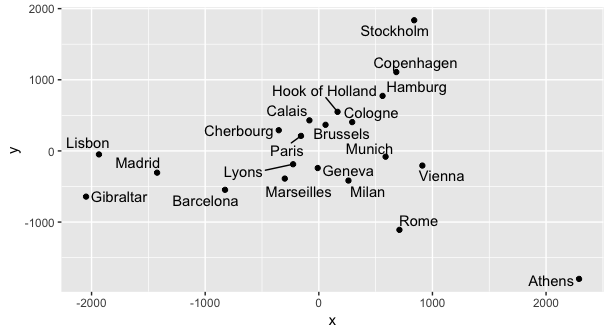
\includegraphics[scale = 0.5]{./images/europ_cities.png}
    \caption{MDS on the European cities.}
    \label{europ_cities}
\end{figure}


\section{Principal coordinates}
Given a matrix \textbf{X} $n \times p$, the matrix of $n$ 
individuals over $p$ variables, it is possible to obtain a new one with 
mean equal to 0 by column from the previous one:

\[
\mathbf{\widetilde{X}} = \Big( \mathbf{I} - \frac{1}{n} \mathbf{1}\mathbf{1'}\Big) \mathbf{X} = \mathbf{P}\mathbf{X},
\]
where 

\[
\mathbf{P} = \Big( \mathbf{I} - \frac{1}{n} \mathbf{1}\mathbf{1'}\Big).
\]

\indent This new matrix, $\mathbf{\widetilde{X}}$, has the same dimensions as 
the original one but its columns mean is \textbf{0}. From this matrix, it is 
possible to build two square semi-positive definite matrices: the covariance 
matrix \textbf{S}, defined as $\mathbf{\widetilde{X}'}\mathbf{\widetilde{X}}/n$ 
and the cross-products matrix $Q = \mathbf{\widetilde{X}}\mathbf{\widetilde{X}'}$. 
The last matrix can be interpreted as a similarity matrix between the $n$ elements. 
The term $ij$ is obtained as follows:

\begin{equation} \label{qij}
q_{ij} = \sum_{s=1}^{p} x_{is}x_{js} = \mathbf{x_i'} \mathbf{x_j}
\end{equation}
where $\mathbf{x_i}'$ is the i-th row from $\mathbf{\widetilde{X}}$. 

\indent Given the scalar product formula, 
${\mathbf{x_i'}\mathbf{x_j} =  \mid \mathbf{x_i} \mid \mid \mathbf{x_i} \mid \cos\theta_{ij}}$,
if the elements $i$ and $j$ have similar coordinates, then $\cos\theta_{ij} \simeq 1$
and $q_{ij}$ will be large. On the contrary, if the elements are very different,
then $\cos \theta_{ij} \simeq 0$ and $q_{ij}$ will be small. So, 
$\mathbf{\widetilde{X}}\mathbf{\widetilde{X}'}$ can be interpreted as the similarity
matrix between the elements.

\indent The distances between elements can be deduced from the similarity 
matrix. The Euclidean distance between two elements is calculated in the 
following way:

\begin{equation} \label{dij}
d^2_{ij} =  \sum_{s=1}^{p} (x_{is}- x_{js} )^2  = \sum_{s=1}^{p}x_{is}^2 + \sum_{s=1}^p x_{js}^2 - 2\sum_{s=1}^{p} x_{is}x_{js}.
\end{equation}

\indent This expression can be obtained directly from the matrix \textbf{Q}:

\begin{equation} \label{dfromq}
d^2_{ij} = q_{ii} + q_{jj} - 2q_{ij}.
\end{equation}

\indent We have just seen that, given the matrix $\mathbf{\widetilde{X}}$, 
it is possible to get the similarity matrix 
$\mathbf{Q} = \mathbf{\widetilde{X}}\mathbf{\widetilde{X}'}$ and from it, 
to get the distance matrix \textbf{D}. Let $\diag(\mathbf{Q})$ be the
vector that contains the diagonal terms of \textbf{Q} and \textbf{1} be the vector
of ones, the matrix \textbf{D} is given by

\[
\mathbf{D} = \diag(\mathbf{Q}) \mathbf{1}' + \mathbf{1}\diag(\mathbf{Q})' - 2\mathbf{Q}.
\]

\indent The problem we are dealing with goes in the opposite direction. We want 
to rebuild $\mathbf{\widetilde{X}}$ from a square distance matrix \textbf{D}, 
with elements $d_{ij}^2$. The first step is to obtain \textbf{Q} and afterwards, 
to get $\mathbf{\widetilde{X}}$. The theory needed to get the solution can be 
found in \cite{pena_libro}. Here, we summarise it.

\indent The first step is to find out a way to obtain the matrix \textbf{Q} 
given \textbf{D}. We can assume without loss of generality that the mean of 
the variables is equal to 0. This is a consequence of the fact that the distance 
between two points remains the same if the variables are expressed in terms 
of the mean:


\begin{equation} \label{dtraslated}
d_{ij}^2 = \sum_{s = 1}^p (x_{is} - x_{js})^2 = \sum_{s=1} ^p [(x_{is} - \overline{x_s})- (x_{js} - \overline{x_s})]^2.
\end{equation}

\indent The previous condition means that we are looking for a matrix  
$\mathbf{\widetilde{X}}$ such that $\mathbf{\widetilde{X}'}\mathbf{1} = 0$. 
It also means that $\mathbf{Q}\mathbf{1} = 0$, i.e, the sum of all the elements 
of a column of \textbf{Q} is 0. Since the matrix is symmetric, the previous 
condition should state for the rows as well. 

\indent To establish these constrains, we sum up (\ref{dfromq}) at row level:

\begin{equation} \label{sumrows}
\sum_{i = 1}^n d_{ij}^2 = \sum_{i = 1}^n q_{ii} + nq_{jj} = t + nq_{jj}
\end{equation}
where $t = \sum_{i = 1}^n q_{ii} = \Tr(\mathbf{Q})$, and we have used that the
condition \textbf{Q}\textbf{1} = 0 implies $\sum_{i = 1}^n q_{ij} = 0$. Summing 
up (\ref{dfromq}) at column level:

\begin{equation} \label{sumcols}
\sum_{j = 1}^n d_{ij}^2 = t + nq_{ii}.
\end{equation}

\indent Summing up (\ref{sumrows}) we obtain:

\begin{equation} \label{doublesum}
\sum_{i = 1}^n\sum_{j = 1}^n d_{ij}^2 = 2nt
\end{equation}

\indent Replacing in (\ref{dfromq}) $q_{jj}$ obtained in (\ref{sumrows}) and $q_{ii}$
obtained in (\ref{sumcols}), we have the following expression:

\begin{equation} \label{generaldij}
d_{ij}^2 = \frac{1}{n}\sum_{i = 1}^n d_{ij}^2 - \frac{t}{n} + \frac{1}{n} \sum_{j = 1}^n d_{ij}^2 -\frac{t}{n} -2q_{ij}
\end{equation}

\indent Let $d_{i.}^2 = \frac{1}{n}\sum_{j = 1}^n d_{ij}^2$ and $d_{.j}^2 = \frac{1}{n}\sum_{i=1}^n d_{ij}^2$ 
be the row-mean and column-mean of the elements of \textbf{D}. Using 
(\ref{doublesum}), we have that

\begin{equation} \label{dmeans}
d_{ij}^2 = d_{i.}^2 + d_{.j}^2 - d_{..}^2-2q_{ij}
\end{equation}
where $d_{..}$ is the mean of all the elements of \textbf{D}, given by

\[
d_{..}^2 = \frac{1}{n^2}\sum \sum d_{ij}^2.
\]

\indent Finally, from (\ref{dmeans}) we get the expression:

\begin{equation} \label{qij2}
q_{ij} = -\frac{1}{2}(d_{ij}^2 - d_{i.}^2 - d_{.j}^2 + d_{..}^2).
\end{equation}

\indent The previous expression shows how to build the matrix of similarities 
\textbf{Q} from the distance matrix \textbf{D}.

\indent The next step is to obtain the matrix \textbf{X} given the matrix 
\textbf{Q}. Let's assume that the similarity matrix is positive definite of 
range $p$. Therefore, it can be represented as

\[
\mathbf{Q} = \mathbf{V}\mathbf{\Lambda}\mathbf{V'}
\]
where $\mathbf{V}$ is a $n \times p$ matrix that contains the eigenvectors with
not nulls eigenvalues of \textbf{Q}. $\mathbf{\Lambda}$ is a diagonal matrix 
$p \times p$ that contains the eigenvalues.

\indent Re-writing the previous expression, we obtain

\begin{equation} \label{generalQ}
\mathbf{Q} = (\mathbf{V}\mathbf{\Lambda}^{1/2})(\mathbf{\Lambda}^{1/2}\mathbf{V'}).
\end{equation}

Getting

\[
\mathbf{Y} = \mathbf{V}\mathbf{\Lambda}^{1/2}.
\]

We have obtained a matrix with dimensions $n \times p$ with $p$ uncorrelated
variables that reproduce the initial metric. It is important to notice that if 
one starts from \textbf{X} (i.e \textbf{X} is known) and calculates from these
variables the distance matrix in (\ref{dij}) and after that it is applied
the method explained, the matrix obtained is not the same as \textbf{X}, but
its principal components. This happens since the distance between the rows in
a matrix does not change if:

\begin{itemize}
\item The row-mean values are modified by adding the same row vector to all
the rows in \textbf{X}.
\item Rows are rotated, i.e, \textbf{X} is postmultiplied by an orthogonal 
matrix.
\end{itemize}

\indent By (\ref{dfromq}), the distance is a function of the terms of the 
similarity matrix \textbf{Q} and this matrix is invariant given any rotation,
reflection or translation of the variables

\[
\mathbf{Q} = \mathbf{\widetilde{X}} \mathbf{\widetilde{X'}} = \mathbf{\widetilde{X}} \mathbf{A} \mathbf{A'}\mathbf{\widetilde{X'}}
\]
for any orthogonal \textbf{A} matrix. The matrix \textbf{Q} only contains 
information about the space generated by the variables \textbf{X}. Any rotation,
reflection or translation preserves the distance. Therefore, the solution
is not unique.


\section{Building principal coordinates}
Let \textbf{D} be a square distance matrix. The process to obtain 
the \textit{principal coordinates} is as follows:

\begin{enumerate}
\item Build the matrix $\mathbf{Q = - \frac{1}{2} PDP}$ of cross-products.
\item Obtain the eigenvalues of \textbf{Q}. Take the $r$ greatest eigenvalues. 
Since $\mathbf{P1}=0$, where \textbf{1} is a vector of ones, 
$\range(\mathbf{Q})=n-1$, being the vector \textbf{1} an eigenvector with 
eigenvalue 0. 
\item Obtain the coordinates of the rows in the variables 
$\mathbf{v_i}\sqrt{\lambda_i}$,
where $\lambda_i$ is an eigenvalue of \textbf{Q} and $\mathbf{v_i}$ is the
associated unitary eigenvector. This implies that \textbf{Q} is approximated by

\[
\mathbf{Q} \approx (\mathbf{V_r \Lambda}^{1/2})(\mathbf{\Lambda_r}^{1/2} \mathbf{V_r'}).
\]

\item Take as coordinates of the points the following variables:
\[
\mathbf{Y_r} = \mathbf{V_r}\mathbf{\Lambda_r}^{1/2}.
\]
\end{enumerate}

\indent The method can also be applied if the initial information is not a 
distance matrix but a similarity matrix. A \textit{similarity function} 
is characterized by the following properties ($s_{ij}$ denotes the
similarity between element $i$ and $j$):


\begin{itemize}
\item $s_{ii} = 1$.
\item $0 \leq s_{ij} \leq 1$.
\item $s_{ij} = s_{ji}$.
\end{itemize}

If the initial information is \textbf{Q}, a similarity matrix, then $q_{ii} = 1$,
$q_{ij} = q_{ji}$ and $0 \leq q_{ij} \leq 1$. The associated distance matrix 
is

\[
d_{ij}^2 = q_{ii} + q_{jj} - 2q_{qij} = 2(1-q_{ij}),
\]
and it is easy to see that $\sqrt{2(1-q_{ij})}$ is a distance and it verifies
the triangle inequality.


\section{Procrustes transformation}
As we have mentioned before, the MDS solution is not unique. One example of it 
is shown in Figure \ref{twosol}.

\begin{figure}[!ht]
    \centering
    \subfloat[]{{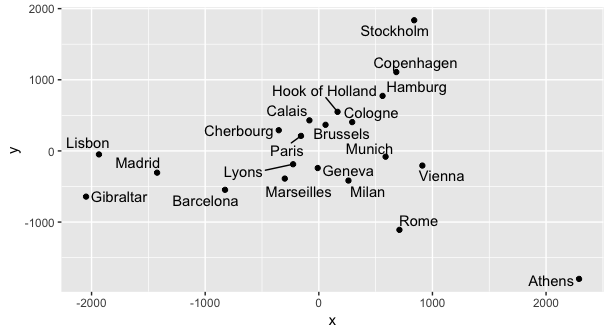
\includegraphics[width=8cm]{./images/europ_cities.png} }}%
    \qquad
    \subfloat[]{{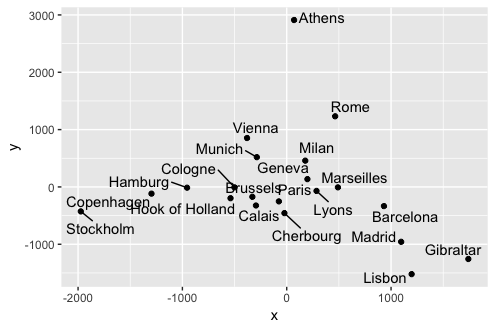
\includegraphics[width=8cm]{./images/europ_cities_rot.png} }}%
    \caption{Two different solutions of MDS.}%
    \label{twosol}%
\end{figure}


\indent Since rotations, translations and reflections are distance-preserving 
functions, one can find two different MDS configurations 
for the same set of data. How is it possible to align both solutions? 
\textit{Align both solutions} (or multiple ones) means to find a common 
coordinate system for all the solutions, i.e, let \textbf{MDS$_1$} and 
\textbf{MDS$_2$} be two MDS solutions of dimensions $n \times r$. We say they 
are aligned if the coordinates of row $i$ are the same in both solutions:

\[
mds_{i1}^1 = mds_{i1}^2, \dots, mds_{ir}^1 = mds_{ir}^2
\]
where $mds_{ij}^k$ is the coordinates $j$ for the individual $i$ given the 
solution $k$, $j \in \{1, \dots r\}$, $i \in \{1, \dots, n\}$ and 
$k \in \{1,2\}$.


\indent This problem is solved by means of \textit{Procrustes transformations}.  
The Procrustes problem is concern with fitting a configuration (testee)
to another (target) as closely as possible. In the simple case, both 
configurations have the same dimensionality and the same number of points, which
can be brought into 1-1 correspondence. Under orthogonal transformations, 
the testee can be fitted it to the target. In addition to such rigid motions, 
one may also allow for dilations and for shifts.

\indent All the details are developed in  \citeN{BorgGroenen2005}. This is out 
of the scope of this thesis. However, since it has been a repeatedly used tool, 
we briefly summarise it. 

\indent Let \textbf{A} and \textbf{B} be two different MDS configurations 
of dimensions $n \times t$ for the same set of data. Without loss of generality, 
let's assume that the target is \textbf{A} and the testee is \textbf{B}. 
One wants to obtain $s \in {\rm I\!R}$, 
$\mathbf{T} \in \mbox{M}_{r\times r}({\rm I\!R})$ and 
$\mathbf{t} \in {\rm I\!R}^r$ such that

\[
\mathbf{A} = s \mathbf{B} \mathbf{T} + \mathbf{1t}'
\]
where \textbf{T} is an orthogonal matrix. As mentioned before, 
in \citeN{BorgGroenen2005} are all the details needed to estimate 
these parameters.

\section{Multidimensional Scaling with \textsf{R}}

All the algorithms have been coded in \textsf{R}. We have used two 
packages for developing our MDS approaches:

\begin{itemize}
\item Package: \textsf{stats}. From this one we have used the function 
\textsf{cmdscale} to do the MDS. The output of this function is a list of 
two elements:
\begin{itemize}
\item The first $r$ principal coordinates for the individuals, i.e,
the low-dimensional configuration for the data.
\item All the eigenvalues found. If the dimensions of the initial dataset 
are $n \times k$, then there are $n$ eigenvalues.
\end{itemize}
\item Package: \textsf{MCMCpack}. From this one we have used the function 
\textsf{procrustes} to do the Procrustes transformation. The output of 
this function is a list of three elements:
\begin{itemize}
\item The dilation coefficient $s$.
\item The orthogonal matrix \textbf{T}.
\item The translation vector \textbf{t}.
\end{itemize}
\end{itemize}

\chapter{Algorithms for Multidimensional Scaling with Big Data}
\label{alg_mds}

\section{Why is it needed?}
In this chapter we present the algorithms developed so that MDS can be applied
when we are dealing with large datasets. The natural question here is why we need 
them if there are already some implementations. To answer this question, let's 
take a look at the Figures \ref{elapsed_time_mds} and \ref{memory_distance}.

 
\begin{figure}[!ht]
\centering
    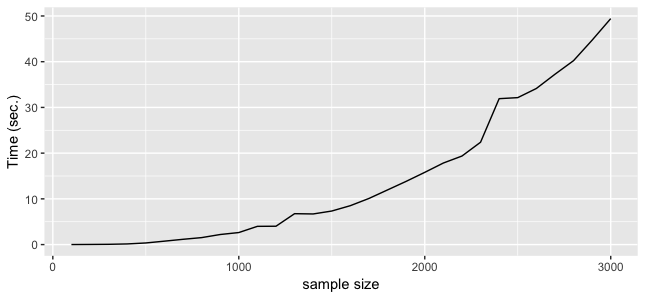
\includegraphics[scale = 0.5]{./images/elapsed_time_mds.png}
    \caption{Elapsed time to compute MDS.}
    \label{elapsed_time_mds}
\end{figure}



\begin{figure}[!ht]
\centering
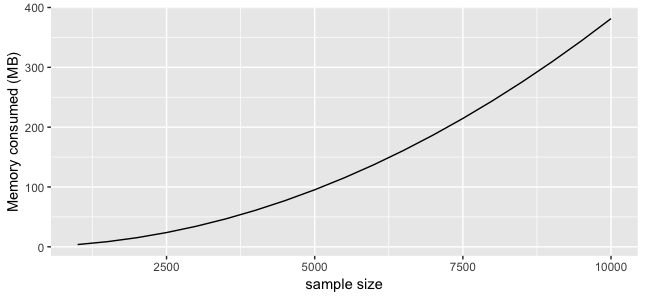
\includegraphics[scale = 0.5]{./images/memory_distance.png}
\caption{Memory consumed to compute distance.}
\label{memory_distance}
\end{figure}


\indent Figure \ref{elapsed_time_mds} shows the time needed to compute MDS
as a function of the sample size. As we can see, the time grows 
considerably as the sample size increases when using \textsf{cmdscale} function. 
Apart of the time issue, there is another one related to the memory needed to 
compute the distance matrix. Figure \ref{memory_distance} points out 
that it is required at least 400MB to store the distance matrix when the 
dataset is close to $10^4$ observations.

\indent In order to solve these problems, we have considered to work on 
three algorithms:


\begin{itemize}
\item \textit{Divide and Conquer MDS:} Before this thesis, 
\textit{Pedro Delicado} had done some work about  MDS with big
datasets and he had already created a first approach, which is this one. The 
algorithm is based on the idea of dividing and conquering. Given a big dataset, 
it is divided into $p$ partitions. After that, MDS is performed over all the 
partitions and, finally, the $p$ solutions are stitched so that all the points 
lie on the same coordinate system.

\item \textit{Fast MDS:} during the phase of gathering information, we found an 
article that solved the problem of scalability \cite{Yang06afast}. The 
authors  use a divide and conquer idea together with recursive programming. 

\item \textit{MDS based on Gower interpolation:} this algorithm uses
Gower interpolation formula, which allows to add a new set of points
to an existing MDS configuration. For further details see, for instance, the 
Appendix of \cite{gowerHand}. 

\end{itemize}

In the next sections we provide a description of the algorithms. 
If further details about the implementation are needed, the code is provided in 
\Cref{chap:code}.

\section{Divide and Conquer MDS}
\subsection{Algorithm}

\begin{itemize}

\item The first step is to divide the original dataset into $p$ partitions: 
$\mathbf{X_1},\dots, \mathbf{X_p}$. The number of partitions, $p$, is also
the number of steps needed to compute the algorithm.

\item Calculate the MDS for the first partition: \textbf{MDS(1)}. This solution
will be used as a guide to align the MDS for the remaining partitions. We 
use a new variable, \textbf{cum-mds}, that will be growing as long as new 
partitions are used. Before adding a new MDS, it is aligned and, after 
that, added. 

\item Define \textbf{cum-mds} equal to \textbf{MDS(1)} and start iterating 
until the last partition is reached.

\item Given a step $k$, $1 < k \leq p$, partitions $k$ and \textit{k-1} are 
joint, i.e, $\mathbf{X_k} \cup \mathbf{X_{k-1}}$. MDS is calculated on 
this union, obtaining $\mathbf{MDS_{k, k-1}}$. In order to add the
rows of the \textit{k-th} partition to \textbf{cum-mds}, the following steps 
are performed:

\begin{itemize}
\item Take the rows of the partition \textit{k-1} from $\mathbf{MDS_{k, k-1}}$: 
$\mathbf{MDS_{k, k-1}} \Bigr|_{k-1}$.
\item Take the rows of the partition \textit{k-1} from \textbf{cum-mds}: 
\textbf{cum-mds} $\Bigr|_{k-1}$.
\item Apply Procrustes to align both solutions. It means that a scalar number
\textit{s}, a vector \textbf{t} and an orthogonal matrix \textbf{T} are obtained
so that
\[
\mathbf{\cummds} \Bigr|_{k-1} \approx s \mathbf{MDS_{k, k-1}} \Bigr|_{k-1} \mathbf{T} + \mathbf{1t'}.
\]
\item Take the rows of the partition $k$ from $\mathbf{MDS_{k, k-1}}: \mathbf{MDS_{k, k-1}} \Bigr|_{k}$.
\item Use the previous Procrustes parameters to add the rows of 
$\mathbf{MDS_{k, k-1}} \Bigr|_{k}$ to \textbf{cum-mds}:
\[
\mathbf{\cummds}_k := s \mathbf{MDS_{k, k-1}} \Bigr|_{k} \mathbf{T} + \mathbf{1t}'.
\]
\item Add the previous dataset to \textbf{cum-mds}, i.e:
\[
\mathbf{\cummds} = \mathbf{\cummds} \cup \mathbf{\cummds}_k
\]

\end{itemize}
\end{itemize}

As we have seen, the algorithm depends on $p$, the number of partitions. How 
many of them are needed? To answer this question, let $l \times l$ be the 
size of the largest matrix that allows to run MDS efficiently, i.e, in a 
reasonable amount of time. If $n$ is the number of rows 
of \textbf{X}, then $p$ is $\frac{2n}{l}$. 

\subsection{Some indicators about the performance of the algorithm}
\label{chap:ind_div}
The aim of this section is to show some indicators about the performance of the
algorithm. A deeper analysis is done in \Cref{chap:sim}, where more details are
provided.

\indent We have generated a matrix \textbf{X} with 3 independent \textit{Normal} 
distributions ($\mu = 0$ and $\sigma = 1$) and $10^3$ rows with $l$ equals to 500. 
Afterwards, we have run the algorithm. We have required the algorithm to 
return 3 columns. So, a new matrix with 3 columns and $10^3$ rows 
($\mathbf{MDS_{Div}}$) has been obtained. Both matrices should be ``equal" 
with an exception of either a rotation, translation or reflection, but 
not a dilation. We have not allowed dilations to see that the distance is 
preserved.

\indent To align the matrices we have performed a Procrustes transformation, but 
setting the the dilation parameter (\textit{s}) equal to 1. 
After that, we have compared the three columns (we refer to the columns as 
\textit{dimensions}). Figure \ref{divide_example} shows the dimension
$i$ of \textbf{X} against the dimension $i$ of $\mathbf{MDS_{Div}}$, 
$i \in \{1,2,3\}$. 

\indent As we can see, the algorithm is able to capture the dimensions of the 
original matrix. We do not show cross-dimensions (i.e dimension $i$ of \textbf{X}
against dimension $j$ of $\mathbf{MDS_{Div}}$ $ i \neq j$), but Table 
\ref{corr_mds} contains the cross-correlation matrix. The results 
show that dimension  $i$ of  $\mathbf{MDS_{Div}}$ captures dimension 
$i$ of \textbf{X} and just dimension $i$. So, it seems that the algorithm, for 
this particular case, has a good performance.


\begin{figure}[!ht]
    \centering
    \subfloat[]{{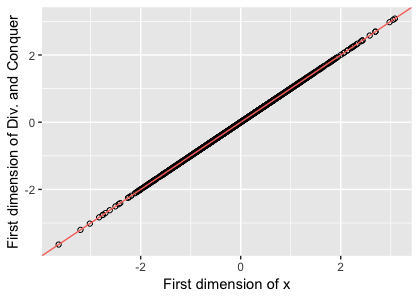
\includegraphics[width=4cm, height=4cm]{./images/first_div.png} }}%
    \qquad
    \subfloat[]{{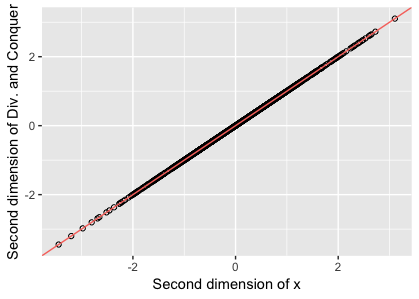
\includegraphics[width=4cm, height=4cm]{./images/second_div.png} }}%
    \qquad
    \subfloat[]{{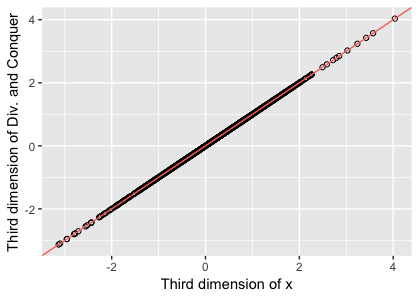
\includegraphics[width=4cm, height=4cm]{./images/third_div.png} }}
    \caption{Dimension 1,2 and 3 of \textbf{X} against dimensions 1,2 and 3 of  $\mathbf{MDS_{Div}}$. \newline
            In red, the line $x=y$.}%
    \label{divide_example}%
\end{figure}


\begin{table}[ht]
\centering
\begin{tabular}{rrrr}
 & 1 & 2 & 3 \\ 
  \hline
1 & 1 & 0.02 & -0.04 \\ 
  2 & 0.02 & 1 & 0.02 \\ 
  3 & -0.04 & 0.02 & 1 \\ 
   \hline
\end{tabular}
\caption{Cross-correlation of \textbf{X} and $\mathbf{MDS_{Div}}$.} 
\label{corr_mds}
\end{table}



\section{Fast MDS}
During the process of gathering information about work previously done around
MDS with big datasets, we found that \citeN{Yang06afast} already proposed an 
algorithm, they named it \textit{Fast Multidimensional Scaling}. 


\subsection{Algorithm}

\begin{itemize}

\item Divide \textbf{X} into $\mathbf{X_1},\dots, \mathbf{X_p}$.

\item Compute MDS for each $\mathbf{X_i}$: 
$\mathbf{MDS_1}, \dots, \mathbf{MDS_p}$. These individuals MDS solutions are 
stitched together by sampling $s$ points (rows) from each submatrix 
$\mathbf{X_i}$ and putting them into an alignment matrix 
$\mathbf{M_{align}}$ of size $sp \times sp$. In principle, $s$ should be at 
least 1 plus the estimated dimensionality of the dataset. In practice, they 
oversample by a factor of 2 or more. 

\item MDS is run on $\mathbf{M_{align}}$. After this, it is obtained
$\mathbf{mMDS}$. Given a sampled point, there are two solutions of MDS: 
one from $\mathbf{X_i}$ and another one from $\mathbf{M_{align}}$.

\item The next step is to compute the Procrustes transformation to  line  
these two sets of solutions up in a common coordinate system:

\[
\mathbf{mMDS_i} = s_i \mathbf{dMDS_i} \mathbf{T_i} + \mathbf{1t_i}'
\]
where:

\begin{itemize}

\item $\mathbf{dMDS_i}$ is $\mathbf{MDS_i}$ but taking into account just
the subset of the sample points that belongs to partition $i$.

\item $\mathbf{mMDS_i}$ is $\mathbf{mMDS}$ but taking into account just
the subset of the sample points that belongs to partition $i$
\end{itemize}

\item After doing the previous part, we obtain a set of $p$ Procrustes 
parameters $(s_i, \mathbf{T_i},  \mathbf{t_i})$. So, the next step is to 
apply this set of parameters to each $\mathbf{MDS_i}$, i.e, 

\[
\mathbf{MDS_i}^a := s_i \mathbf{MDS_i} \mathbf{T_i} + \mathbf{1t_i'}.
\]

\item The last step is to join $\mathbf{MDS_1}^a, \dots,  \mathbf{MDS_p}^a$ 
all together, i.e, 
\[
\mathbf{MDS_X}:= \mathbf{MDS_1}^a \cup \cdots \cup \mathbf{MDS_p}^a.
\]

\end{itemize}

\indent They apply this process recursively until the size of $\mathbf{X_i}$ is
optimal to run MDS on. They find the stop condition as follows. Let 
$l \times l$ be the size of the largest matrix that allow MDS to be executed 
efficiently, i.e, in a reasonable amount of time. There are two issues that 
impact the performance of the algorithm: the size of each submatrix after 
subdivision and the number of submatrices, $p$, that are stitched together 
at each step. Ideally, the size of each submatrix after division should 
be as large as possible without exceeding $l$. By the same token, the size of 
$\mathbf{M_{align}}$ should be bounded by $l$. The number of 
submatrices to be stitched together, $p$, should be the largest number such 
that $sp \leq l$.

\subsection{Some indicators about the performance of the algorithm}
As we have done in \Cref{chap:ind_div}, we present some visual results of
this algorithm. The data used are the same as in \Cref{chap:ind_div}. We
call $\mathbf{MDS_{Fast}}$ the result that provides the previous algorithm.

\indent Figure \ref{fast_example} shows that, for this particular case,
the algorithm captures quite well the dimensions of the original data, 
providing a good performance. In addition, dimension $i$ of 
$\mathbf{MDS_{Fast}}$ fits perfectly the same dimensions $i$ of \textbf{X} and 
just this one, as we can see in Table \ref{corr_fast}.


\begin{figure}[!ht]
    \centering
    \subfloat[]{{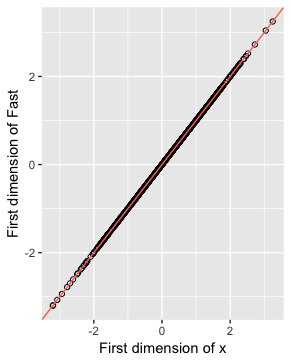
\includegraphics[width=4cm, height=4cm]{./images/first_fast.png} }}%
    \subfloat[]{{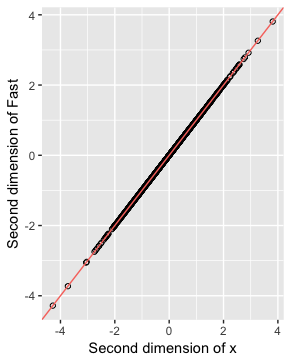
\includegraphics[width=4cm, height=4cm]{./images/second_fast.png} }}%
    \subfloat[]{{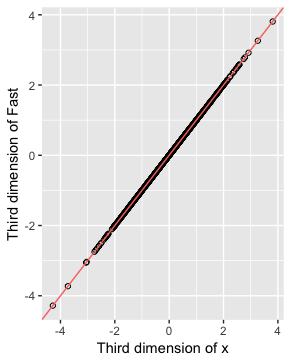
\includegraphics[width=4cm, height=4cm]{./images/third_fast.png} }}
    \caption{Dimensions 1,2 and 3 of \textbf{X} against dimensions 1,2 and 3 of  $\mathbf{MDS_{Fast}}$. \newline
            In red, the line $x=y$.}%
    \label{fast_example}%
\end{figure}


\begin{table}[ht]
\centering
\begin{tabular}{rrrr}
 & 1 & 2 & 3 \\ 
  \hline
  1 & 1 & 0.02 & 0 \\ 
  2 & 0.02 & 1 & 0.02 \\ 
  3 & 0 & 0.02 & 1 \\ 
   \hline
\end{tabular}
\caption{Cross-correlation of \textbf{X} and $\mathbf{MDS_{Fast}}$.} 
\label{corr_fast}
\end{table}

\section{MDS based on Gower interpolation}

Gower interpolation formula (see Appendix of \cite{gowerformula}) allows to add 
a new set of points to a given MDS configuration. Given a matrix 
\textbf{X} $n \times p$, a MDS configuration for this matrix of dimension 
$n \times c$ and a matrix $\mathbf{X_{new}}$ $m \times p$, one wants to 
add these new $m$ rows to the existing MDS configuration. So, 
after adding this new rows, the MDS configuration will have $n+m$ rows and 
$c$ columns. We briefly summarise how to do so:

\begin{itemize}

\item Obtain $\mathbf{J} = \mathbf{I_n} - \frac{1}{n}\mathbf{1}\mathbf{1}'$,
where $\mathbf{I_n}$ is the identity matrix $n \times n$.

\item Given the distance matrix \textbf{D} of the rows of \textbf{X},
calculate $\mathbf{\Delta} = (\delta_{ij}^2)$.

\item Calculate $\mathbf{G} = - \frac{1}{2} \mathbf{J} \mathbf{\Delta} \mathbf{J}'$

\item Let \textbf{g} be the diagonal of \textbf{G}, i.e, 
$\mathbf{g} = \diag({\mathbf{G}})$. We treat \textbf{g} as a vector. 

\item Let \textbf{A} be the distance matrix between the rows of 
\textbf{X} and the rows of $\mathbf{X_{new}}$. \textbf{A} has dimensions 
$m \times n$. Let $\mathbf{A}^2$ be the matrix of the square elements 
of \textbf{A}, i.e, $\mathbf{A}^2 = (a_{ij}^2)$.

\item Let \textbf{M} and \textbf{S} be the MDS for \textbf{X} and the 
variance-covariance matrix of the $c$ columns of \textbf{M}.

\item The interpolated coordinates for the new $m$ observations are given by

\begin{equation} \label{gower_f}
\frac{1}{2n} (\mathbf{1}\mathbf{g}' - \mathbf{A}^2) \mathbf{M}\mathbf{S}^{-1}.
\end{equation}

\end{itemize}

The resulting MDS for the $m$ observations of $\mathbf{X_{new}}$ is in the same
coordinate system as \textbf{M}. So, here it is not needed to do any 
Procrustes transformation.

\subsection{Algorithm}

\begin{itemize}
\item Divide \textbf{X} into $p$ partitions $\mathbf{X_1},\dots, \mathbf{X_p}$.
We use the procedure explained above, being $\mathbf{X_{new}} := \mathbf{X_k}$,
$k \in \{1, \dots, p\}$.

\item Calculate \textbf{J}, $\mathbf{\Delta}$, \textbf{G}, \textbf{g},
\textbf{A}, \textbf{M} and \textbf{S} according to the above formulas.

\item Obtain MDS for the first partition $\mathbf{X_1}$. 

\item Given a partition $1 < k \leq p$, do the following steps to get the 
related MDS:

\begin{itemize}

\item Calculate the distance matrix between the rows of $\mathbf{X_1}$ and
$\mathbf{X_k}$ and calculate the square of each element of this matrix. Let
$\mathbf{A}^2$ be this matrix (same as above).

\item Use Gower interpolation formula (\ref{gower_f}) to obtain MDS for 
partition $k$. 

\item Accumulate this solution.


\end{itemize}

\end{itemize}


As in the previous two algorithms, there is a key parameter to choose: $p$,
the number of partitions. For this algorithm, $p$ is set in the following way.
Let $l \times l$ be the size of the largest distance matrix that a computer can 
calculate efficiently, i.e, in a reasonable amount of time. The value of 
$p$ is set as $n/p$.


\subsection{Some indicators about the performance of the algorithm}
We repeat the same as in \Cref{chap:ind_div}. Figure \ref{gower_example} 
and Table \ref{corr_gower} shows that the algorithm, for this particular case, 
captures quite well the dimensions of the original data, providing a 
good performance.

\begin{figure}[!ht]
    \centering
    \subfloat[]{{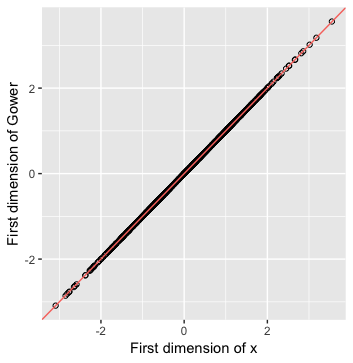
\includegraphics[width=4cm, height=4cm]{./images/first_gower.png} }}%
    \subfloat[]{{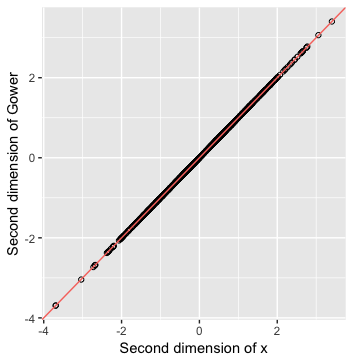
\includegraphics[width=4cm, height=4cm]{./images/second_gower.png} }}%
    \subfloat[]{{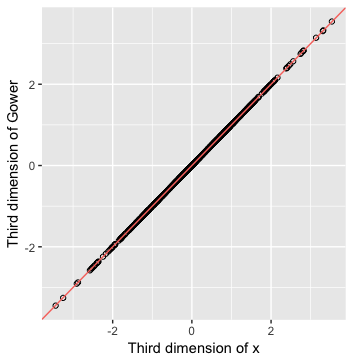
\includegraphics[width=4cm, height=4cm]{./images/third_gower.png} }}
    \caption{Dimensions 1,2 and 3 of \textbf{X} against dimensions 1,2 and 3 of  $\mathbf{MDS_{Gower}}$. \newline
            In red, the line $x=y$.}%
    \label{gower_example}%
\end{figure}


\begin{table}[ht]
\centering
\begin{tabular}{rrrr}
 & 1 & 2 & 3 \\ 
  \hline
  1 & 1 & 0 & -0.04 \\ 
  2 & 0 & 1 & -0.0 \\ 
  3 & -0.04 & -0.03 & 1 \\ 
   \hline
\end{tabular}
\caption{Cross-correlation of \textbf{X} and $\mathbf{MDS_{Gower}}$.} 
\label{corr_gower}
\end{table}


\section{Comparison of the algorithms}
\indent The three previous algorithms share the same goal: obtaining a MDS 
configuration for a given big dataset. However, there are some differences 
between the approaches that impact the performance of the algorithms. 
The main differences between them are:

\begin{itemize}
\item \textit{Divide and Conquer MDS} uses a guide 
(the first subset, $\mathbf{X_1}$) to align the solutions as well as it uses the whole partition $\mathbf{X_i}$ to find the Procrustes parameters. However, 
\textit{Fast MDS} does not use a guide an it uses a set of subsamples to 
find the Procrustes parameters.

\item \textit{Fast MDS} is based on recursive programming. It divides until 
a manageable dimensionality is found. However, \textit{Divide and Conquer MDS} 
finds the number of partitions without applying recursive programming.

\item \textit{MDS based on Gower interpolation} does not need any Procrustes
transformation. 

\end{itemize}

The fact that we found three algorithms to compute MDS possesses some questions 
that need to be answered:

\begin{itemize}
\item Are these algorithms able to capture the data dimensionality as good as 
classical MDS does?
\item Which is the fastest method?
\item Can they deal with big datasets in a reasonable amount of time?
\item How are they performing when dealing with big data sets?
\end{itemize}

All these questions and are answered in \Cref{chap:sim}.

\section{Output of the algorithms}
The three algorithms have the same type of output. It consists on a list of 
two parameters. 

\indent The first parameter is the MDS configuration calculated by the 
algorithm. It is a matrix of $n$ rows and $c$ columns, where $n$ is the number 
of rows of the input data and $c$ is the number of dimensions the user has 
required.

\indent The second parameter is a list of eigenvalues. This list is built
as follows: 

\begin{itemize}
\item All the algorithms divide the initial data into a set of $p$ partitions.

\item Given a partition $i$, a distance matrix of dimensions $m_i \times m_i$
is calculated: $\mathbf{D_i}$. 

\item Over $\mathbf{D_i}$ a singular value decomposition is performed, providing 
a list of length $m_i$ that contains all the eigenvalues of the previous 
decomposition: $list_i$.

\item Let $norm\_eigenvalues_i$ be $list_i/m_i$, i.e, each eigenvalue is divided
by the number of rows of $\mathbf{D_i}$.

\item The algorithms return 
$norm\_eigenvalues_1 \cup \cdots \cup norm\_eigenvalues_p$. We refer to 
this union as the \textit{normalized eigenvalues}. 

\end{itemize}





\chapter{Simulation study}
\label{chap:sim}

\section{Design of the simulation}


Given the three algorithms, we would like to know how they perform. There 
are two issues to study:

\begin{itemize}
\item Performance of the algorithms: are they able to capture data
dimensionality?
\item Performance in terms of time: are they `` fast" enough? Which one is 
the fastest?
\end{itemize}

To test the algorithms under different conditions, a simulation study has been
carried out. The scenarios are obtained as combinations of:

\begin{itemize}
\item \textit{Sample size}: we use different sample sizes, combining small
data sets and big ones. A total of six sample sizes are used, which are:
$10^3, 3\cdot 10^3, 5\cdot10^3, 10^4, 10^5, 10^6$.

\item \textit{Data dimensions}: we generate a matrix with two different number 
of columns: 10, 100.

\item \textit{Main dimensions}: given the data matrix \textbf{X} $n \times k$\footnote{$n \in \{10^3, 3\cdot 10^3, 5\cdot10^3, 10^4, 10^5, 10^6 \}$ and $k \in \{10, 100\}$},
it is postmultiplied by a diagonal matrix that contains $k$ values, 
$\lambda_1, \dots, \lambda_k$. The first values are much higher than the rest.
The idea of this is to see if the algorithms are able to capture the main
dimensions of the original dataset, i.e, the columns  with the highest variance. 
We set 5 combinations for this variable, which are:

\begin{itemize}
\item All the columns with the same values of $\lambda$: 
$\lambda_1 = \cdots = \lambda_k = 1$.

\item One main dimension with $\lambda_1 = 15$ and 
$\lambda_2 = \cdots = \lambda_k = 1$.

\item  Two main dimensions of the same value $\lambda$: 
$\lambda_1  = \lambda_2 = 15$, $\lambda_3 = \cdots \lambda_k = 1$.

\item  Two main dimensions of different values $\lambda$: 
$\lambda_1  = 15$, $\lambda_2 =10$, $\lambda_3 = \cdots \lambda_k = 1$.

\item  Four main dimensions of the same value $\lambda$: 
$\lambda_1  = \lambda_2 = \lambda_3 = \lambda_4 = 15$, $\lambda_5 = \cdots \lambda_k = 1$.


\end{itemize}

\item As probabilistic model, we use a Normal distribution with $\mu = 0$ and 
$\sigma = 1$. With this distribution, we generate a matrix of $n$ observations
and $k$ columns, being the $k$ columns independent .After generating the 
dataset \textbf{X}, it is postmultiplied by the diagonal matrix that contains
the values of $\lambda$'s.


\end{itemize}

There is a total of 60 scenarios to simulate. Given a scenario, it is 
replicated 100 times. For every simulation, it is generated a dataset 
(according to the scenario), and all the algorithms are run using this dataset.
So, a total of 6000 simulations are carried out.

\indent Table \ref{scenarios_sim} shows the 
configuration of each scenario. Given a scenario, \textit{scenario\_id} 
identifies it. We refer to a scenario by its \textit{scenario\_id}. 

\begin{longtable}{|r|r|r|r|l|} 
\hline
& scenario\_id & sample\_size & n\_dimensions & value\_primary\_dimensions \\ 
\hline
1 & 1 & $10^3$ & 10 & NULL \\ 
\hline
2 & 2 & $10^3$ & 100 & NULL \\ 
\hline
3 & 3 & $10^3$ & 10 & 15 \\ 
\hline
4 & 4 & $10^3$ & 100 & 15 \\ 
\hline
5 & 5 & $10^3$ & 10 & c(15, 15) \\ 
\hline
6 & 6 & $10^3$ & 100 & c(15, 15) \\ 
\hline
7 & 7 & $10^3$ & 10 & c(15, 10) \\ 
\hline
8 & 8 & $10^3$ & 100 & c(15, 10) \\ 
\hline
9 & 9 & $10^3$ & 10 & c(15, 15, 15, 15) \\ 
\hline
10 & 10 & $10^3$ & 100 & c(15, 15, 15, 15) \\ 
\hline
\hline
11 & 2000 & $3 \cdot 10^3$ & 10 & NULL \\ 
\hline
12 & 2001 & $3 \cdot 10^3$ & 100 & NULL \\ 
\hline
13 & 2002 & $3 \cdot 10^3$ & 10 & 15 \\ 
\hline
14 & 2003 & $3 \cdot 10^3$ & 100 & 15 \\ 
\hline
15 & 2004 & $3 \cdot 10^3$ & 10 & c(15, 15) \\ 
\hline
16 & 2005 & $3 \cdot 10^3$ & 100 & c(15, 15) \\ 
\hline
17 & 2006 & $3 \cdot 10^3$ & 10 & c(15, 10) \\ 
\hline
18 & 2007 & $3 \cdot 10^3$ & 100 & c(15, 10) \\ 
\hline
19 & 2008 & $3 \cdot 10^3$ & 10 & c(15, 15, 15, 15) \\ 
\hline
20 & 2009 & $3 \cdot 10^3$ & 100 & c(15, 15, 15, 15) \\ 
\hline
\hline
21 & 4000 & $5 \cdot 10^3$ & 10 & NULL \\ 
\hline
22 & 4001 & $5 \cdot 10^3$ & 100 & NULL \\ 
\hline
23 & 4002 & $5 \cdot 10^3$ & 10 & 15 \\ 
\hline
24 & 4003 & $5 \cdot 10^3$ & 100 & 15 \\ 
\hline
25 & 4004 & $5 \cdot 10^3$ & 10 & c(15, 15) \\ 
\hline
26 & 4005 & $5 \cdot 10^3$ & 100 & c(15, 15) \\ 
\hline
27 & 4006 & $5 \cdot 10^3$ & 10 & c(15, 10) \\ 
\hline
28 & 4007 & $5 \cdot 10^3$ & 100 & c(15, 10) \\ 
\hline
29 & 4008 & $5 \cdot 10^3$ & 10 & c(15, 15, 15, 15) \\
\hline
30 & 4009 & $5 \cdot 10^3$ & 100 & c(15, 15, 15, 15) \\ 
\hline
\hline
31 & 6000 & $10^4$ & 10 & NULL \\ 
\hline
32 & 6001 & $10^4$ & 100 & NULL \\ 
\hline
33 & 6002 & $10^4$ & 10 & 15 \\ 
\hline
34 & 6003 & $10^4$ & 100 & 15 \\ 
\hline
35 & 6004 & $10^4$ & 10 & c(15, 15) \\ 
\hline
36 & 6005 & $10^4$ & 100 & c(15, 15) \\ 
\hline
37 & 6006 & $10^4$ & 10 & c(15, 10) \\ 
\hline
38 & 6007 & $10^4$ & 100 & c(15, 10) \\ 
\hline
39 & 6008 & $10^4$ & 10 & c(15, 15, 15, 15) \\ 
\hline
40 & 6009 & $10^4$ & 100 & c(15, 15, 15, 15) \\ 
\hline
\hline
41 & 20000 & $10^5$ & 10 & NULL \\ 
\hline
42 & 20001 & $10^5$ & 100 & NULL \\ 
\hline
43 & 20002 & $10^5$ & 10 & 15 \\
\hline
44 & 20003 & $10^5$ & 100 & 15 \\ 
\hline
45 & 20004 & $10^5$ & 10 & c(15, 15) \\ 
\hline
46 & 20005 & $10^5$ & 100 & c(15, 15) \\ 
\hline
47 & 20006 & $10^5$ & 10 & c(15, 10) \\ 
\hline
48 & 20007 & $10^5$ & 100 & c(15, 10) \\ 
\hline
49 & 20008 & $10^5$ & 10 & c(15, 15, 15, 15) \\ 
\hline
50 & 20009 & $10^5$ & 100 & c(15, 15, 15, 15) \\ 
\hline
\hline
51 & 30000 & $10^6$ & 10 & NULL \\ 
\hline
52 & 30001 & $10^6$ & 100 & NULL \\ 
\hline
53 & 30002 & $10^6$ & 10 & 15 \\ 
\hline
54 & 30003 & $10^6$ & 100 & 15 \\ 
\hline
55 & 30004 & $10^6$ & 10 & c(15, 15) \\ 
\hline
56 & 30005 & $10^6$ & 100 & c(15, 15) \\ 
\hline
57 & 30006 & $10^6$ & 10 & c(15, 10) \\ 
\hline
58 & 30007 & $10^6$ & 100 & c(15, 10) \\ 
\hline
59 & 30008 & $10^6$ & 10 & c(15, 15, 15, 15) \\ 
\hline
60 & 30009 & $10^6$ & 100 & c(15, 15, 15, 15) \\ 
\hline
\caption{Scenarios simulated} 
\label{scenarios_sim}
\end{longtable}


\indent Note that scenarios 1, 2, 2000, 2001, 4000, 4001, 6000, 6001, 20000,
20001, 30000, 30001 are pure noise. We refer to them as \textit{noisy 
scenarios}.

\indent In order to test the performance of the algorithms as well as the time
needed to compute the MDS configuration, some metrics are calculated. These
metrics are the following ones:

\begin{itemize}
\item Performance: in terms of performance two metrics are calculated, which 
are:
\begin{itemize}


\item Correlation between the main dimensions of the data and the
main dimensions after applying the algorithms. We get the diagonal of the 
correlation matrix, i.e, the correlation between dimension $i$ of the data 
and the dimension $i$ of the algorithm. 

\item \textit{Normalized eigenvalues} as an approximation of the standard 
deviation of the variables of \textbf{X}.
\end{itemize}

\item Elapsed Time to get the MDS configuration: Given an algorithm, we compute 
and store the elapsed time to get the corresponding MDS configuration.

\end{itemize}

\indent We do it in this way because we want to check some hypothesis. We 
expect the three algorithms to behave ``correctly". By ``correctly" we mean 
that the behavior should be the same as if classical MDS were run. Therefore, 
we expect that the correlation between the main dimensions of the data and the
main dimensions of the MDS of each algorithm is close to 1 when the
dimension asked to MDS is $k$, i.e, the same dimension as the original dataset.

\indent In addition, the variance of the original data should be captured. 
So, given the highest \textit{normalized eigenvalues}, we expect that 
its square root is approximately 15 or 10 when the scenarios are not the 
\textit{noisy scenarios}. 

\indent For the time of the algorithms, we have done some tests and it seems 
that \textit{MDS based on Gower interpolation} seems to be the fastest.
So, it will be tested.


\indent Given a scenario, the steps that we have performed to calculate  and to
store all the data needed are:

\begin{enumerate}

\item Generate the data according to the scenario. 

\item For each algorithm, we do the following steps:

\begin{enumerate}

\item Run the algorithm and get MDS configuration for the algorithm
($\mathbf{MDS_{alg}}$).

\item Get the elapsed time to compute MDS configuration and store it.

\item Get \textit{normalized eigenvalues} and store them.

\item Align $\mathbf{MDS_{alg}}$ and \textbf{X} using Procrustes.

\item Get the correlation coefficients between the main dimensions of 
$\mathbf{MDS_{alg}}$ and \textbf{X} and store it.

\end{enumerate}

\end{enumerate}

\indent There are some important details that affect the results of the 
simulations, which are:

\begin{itemize}

\item When running the algorithms, we ask for as many columns as the original 
data has, i.e, $k$. Therefore, the low-dimensional space has the same 
dimension as the original dataset.

\item For the \textit{normalized eigenvalues}, we just store 6 eigenvalues 
instead of the full list of eigenvalues (otherwise we would store $n$ 
eigenvalues, which is memory consuming). 

\item For Procrustes we dot not allow dilations, otherwise distance could not
be preserved. In addition, we do not use all the columns 
to do the alignment, we select the main dimensions. If there is not any
main dimension, i.e it is one of the \textit{noisy scenarios}, we just select 4 
columns. 

\item To avoid memory problems with the alignment when $n$ is greater or 
equal to $10^5$, Procrustes is done in the following way:

\begin{enumerate}

\item Create $p$ partitions of \textbf{X} and the result of a given MDS 
algorithm ($\mathbf{MDS_{alg}}$). Both sets of partitions contain exactly the
same observations.


\item For each partition get the Procrustes parameters without dilations.

\item Accumulate the parameters iteration after iteration. So, at the end, 
we obtain $\mathbf{R} = \sum_{i = 1}^p \mathbf{R_i}$ and 
$\mathbf{t} = \sum_{i = 1}^p \mathbf{t_i}$.

\item $\mathbf{R} = \mathbf{R}/p$ and $\mathbf{t} = \mathbf{t}/p$.

\item Apply these parameters to $\mathbf{MDS_{alg}}$ so that 
\textbf{X} and $\mathbf{MDS_{alg}}$ are in the same coordinate system and
they can be compared, i.e

\[
\mathbf{X_{Procrustes}} = \mathbf{X} \mathbf{R} + \mathbf{1t'}.
\]


\end{enumerate}
\end{itemize}

\indent The algorithms have as input values a set of variables. The input matrix 
is already explained, but there is another parameter that has been used in 
the description of the algorithms (see \Cref{alg_mds}): $l$. The meaning of 
$l$ is a little bit different in each algorithm, but for simplicity we 
set this value equals to 500. 

\indent \textit{Fast MDS} has an extra parameter: the amplification parameter.
It is used the value that they used to test this algorithm, i.e, a value of
3. So, for each partition, it is taken 30 (when the original matrix
has 10 columns) or 300 (when the original matrix has 100 columns) points for
every partition to build $\mathbf{M_{align}}$.

\indent Finally, there is an extra ``parameter" to take into account: the 
machine used to do the simulations. Since a total of 6000 simulations are
performed and some of them include big datasets, we use 
\textit{Amazon Web Services} (AWS) to carry out the simulations. 
10 servers of the same type are used: \textit{c5n.4xlarge}. It 
has 16 cores and 42 GB of memory RAM. We use this server because it is 
designed for applications like batch and log processing, distributed and or 
real-time analytics. 

\section{Correlation coefficients}
In this section we provide some results for the correlation coefficients based
on the simulations. Given a scenario and its dataset \textbf{X} 
$n \times k$, the correlation matrix between the main dimensions of \textbf{X} 
and the main dimensions of $\mathbf{MDS_{alg}}$ is computed. We are interested
in the diagonal of the correlation matrix, expecting that the values are close
to 1. We expect 1 as a correlation coefficient because the number of dimensions
required to the MDS configuration is the same as the number of dimensions of
the original dataset.

\indent The length of the diagonal correlation matrix is not static. Depending
on the scenario it can be:

\begin{itemize}
\item 1, when  $\lambda_1 = 15$ and $\lambda_2 = \cdots = \lambda_k = 1$.

\item 2, when$\lambda_1  = \lambda_2 = 15$, $\lambda_3 = \cdots \lambda_k = 1$
or $\lambda_1  = 15$, $\lambda_2 =10$, $\lambda_3 = \cdots \lambda_k = 1$.

\item 4, when $\lambda_1  = \lambda_2 = \lambda_3 = \lambda_4 = 15$, 
$\lambda_5 = \cdots \lambda_k = 1$.

\item 0, when $\lambda_1 = \cdots = \lambda_k = 1$, i.e, 
\textit{noisy scenarios}.

\end{itemize}

\indent Figure \ref{divide_correlation_1000} shows some boxplots of the 
correlation coefficients between the main dimensions of the data \textbf{X} 
and the main dimensions of $\mathbf{MDS_{Div}}$, where  $\mathbf{MDS_{Div}}$ is
the MDS configuration for \textit{Divide and Conquer MDS}. As we can see, 
all the values are close to 1, showing a good performance. 


\begin{figure}[!h]
\centering
    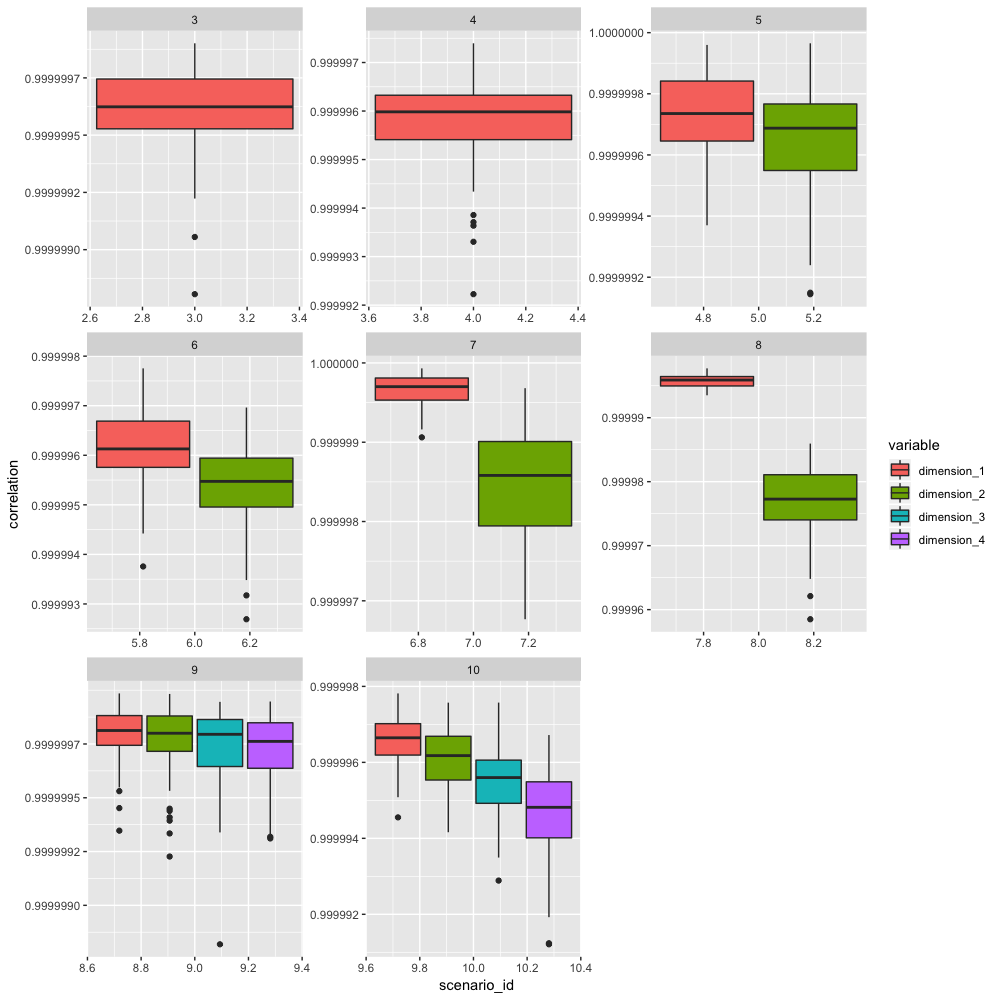
\includegraphics[width=8cm, height=10cm]{./images/divide_correlation_1000.png}
    \caption{Correlation for $n = 10^3$ and MDS Divide and conquer algorithm}
    \label{divide_correlation_1000}
\end{figure}

\begin{figure}[!h]
\centering
    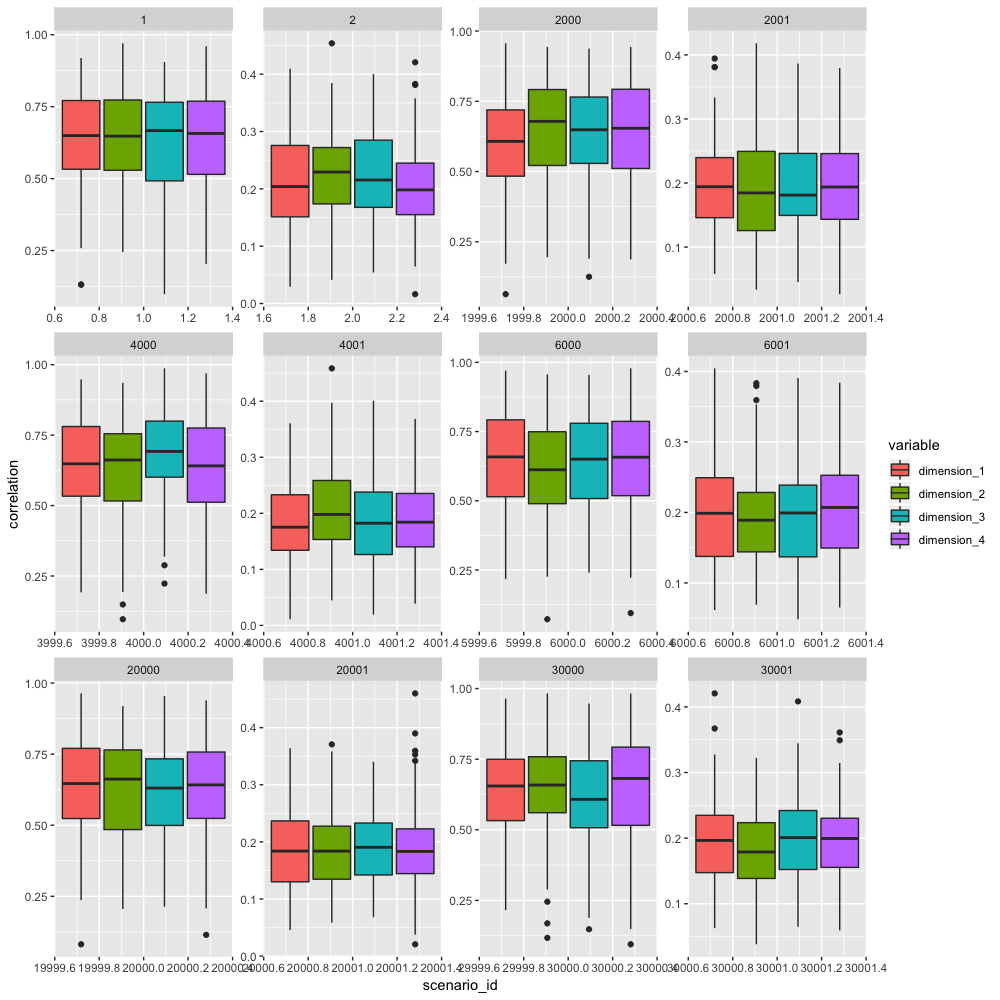
\includegraphics[width=8cm, height=10cm]{./images/divide_correlation_noise.png}
    \caption{Correlation for \textit{noisy scenarios} and MDS Divide and conquer algorithm}
    \label{divide_correlation_noise}
\end{figure}



\indent Note that before calculating the correlation matrix, Procrustes 
transformation is performed (dilations are not allowed) so that both coordinate 
systems are the same.

\indent Figure \ref{divide_correlation_1000} just shows the correlation
coefficients for $n = 10^3$. The remaining figures are in 
\Cref{div_conquer_corr}. All of them have the same shape, independently of the
scenario: there is always a high correlation between the data and the MDS. 
Actually, the correlation is so high that it is not needed any hypothesis test
to check if the value is 1 or not. 

\indent Figure \ref{divide_correlation_noise} shows the boxplot for the 
\textit{noisy scenarios}. It has been taken 4 dimensions to do the alignment, 
instead of all the dimensions (10 or 100). Because of this, we expect a random 
distribution between them within [0,1] interval. If we had taken all the 
dimensions, we would be seeing higher correlation values. 

\indent We do the same for \textit{Fast MDS} algorithm. Figure 
\ref{fast_correlation_1000} shows the boxplot of the correlation coefficients 
between the data and the MDS of this algorithm. Again, there is high correlation 
between them. Figure \ref{fast_correlation_noise} shows the boxplot for the 
\textit{noisy scenarios}. The remaining plots are in \Cref{fast_corr}.


\begin{figure}[!ht]
\centering
    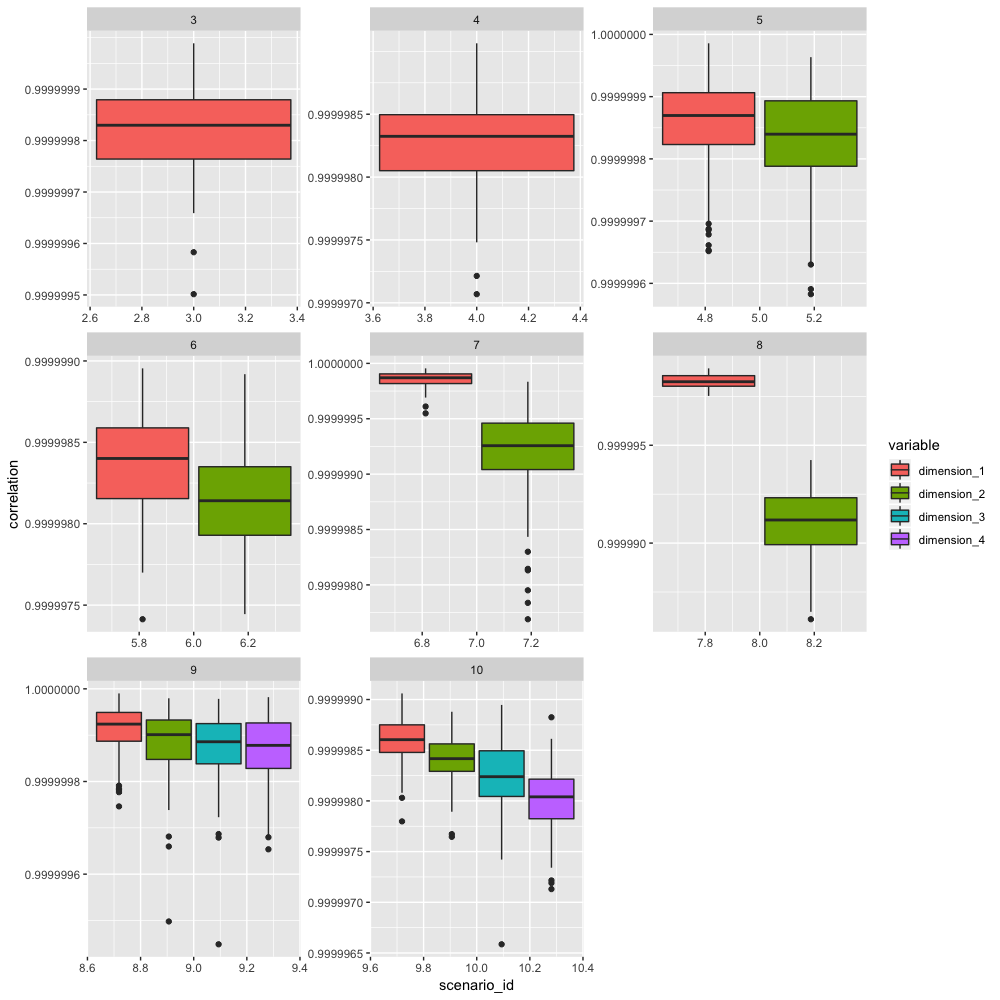
\includegraphics[width=8cm, height=10cm]{./images/fast_correlation_1000.png}
    \caption{Correlation for $n = 10^3$ and MDS Fast algorithm.}
    \label{fast_correlation_1000}
\end{figure}

\begin{figure}[!ht]
\centering
    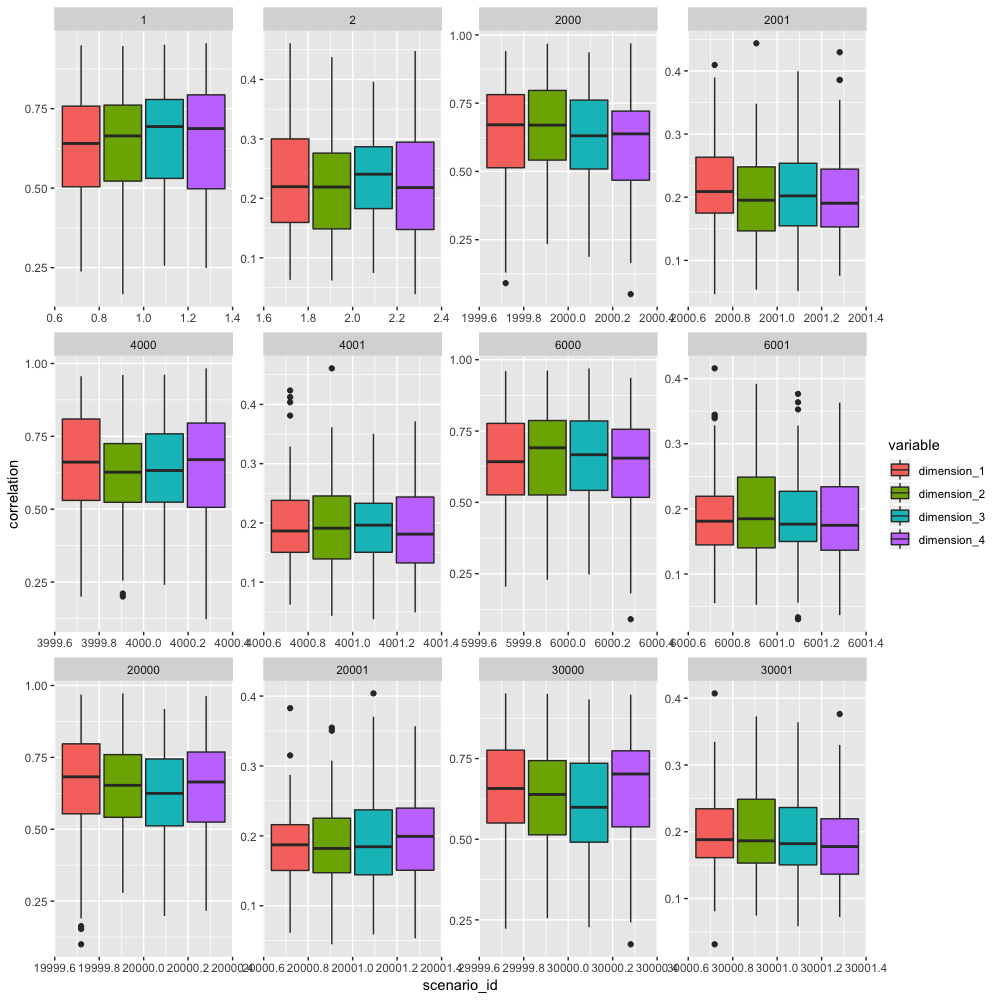
\includegraphics[width=8cm, height=10cm]{./images/fast_correlation_noise.png}
    \caption{Correlation for \textit{noisy scenarios} and MDS Fast algorithm.}
    \label{fast_correlation_noise}
\end{figure}

\begin{figure}[!ht]
\centering
    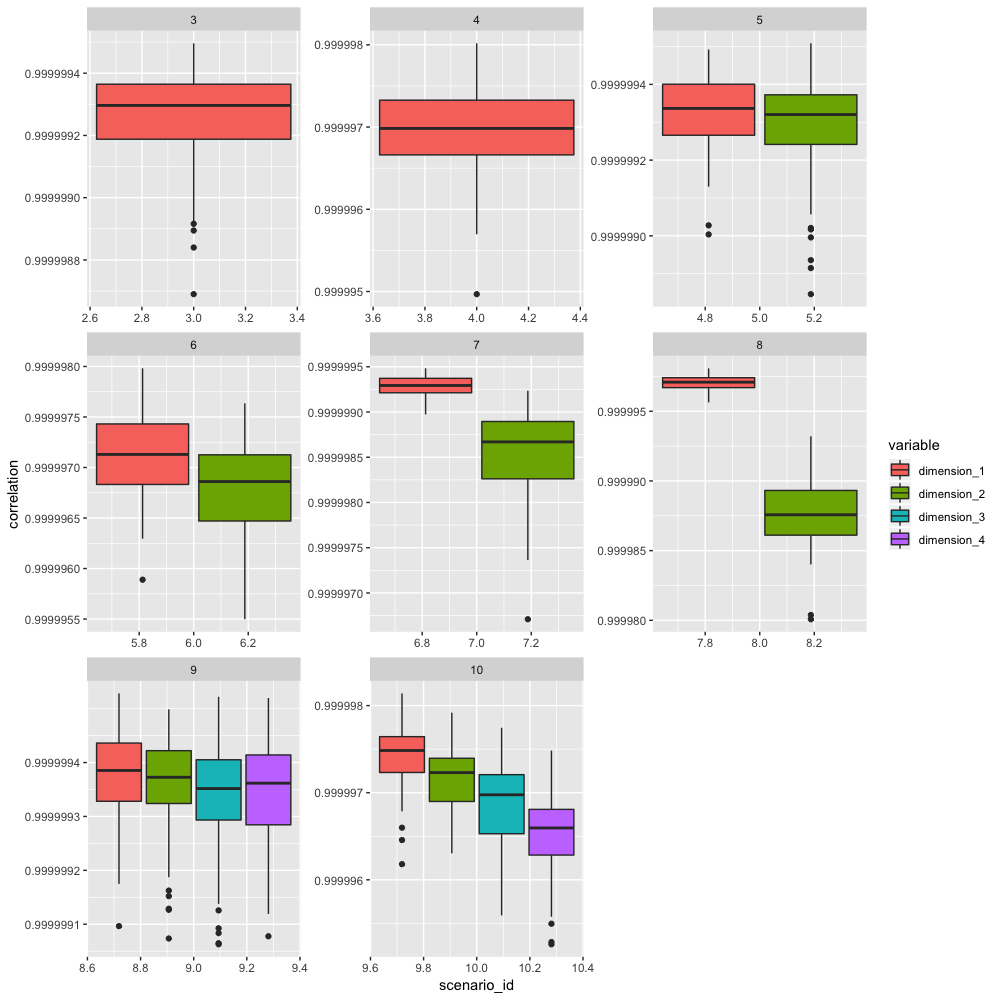
\includegraphics[width=8cm, height=10cm]{./images/gower_correlation_1000.png}
    \caption{Correlation for $n = 10^3$ and MDS based on Gower algorithm.}
    \label{gower_correlation_1000}
\end{figure}

\begin{figure}[!ht]
\centering
    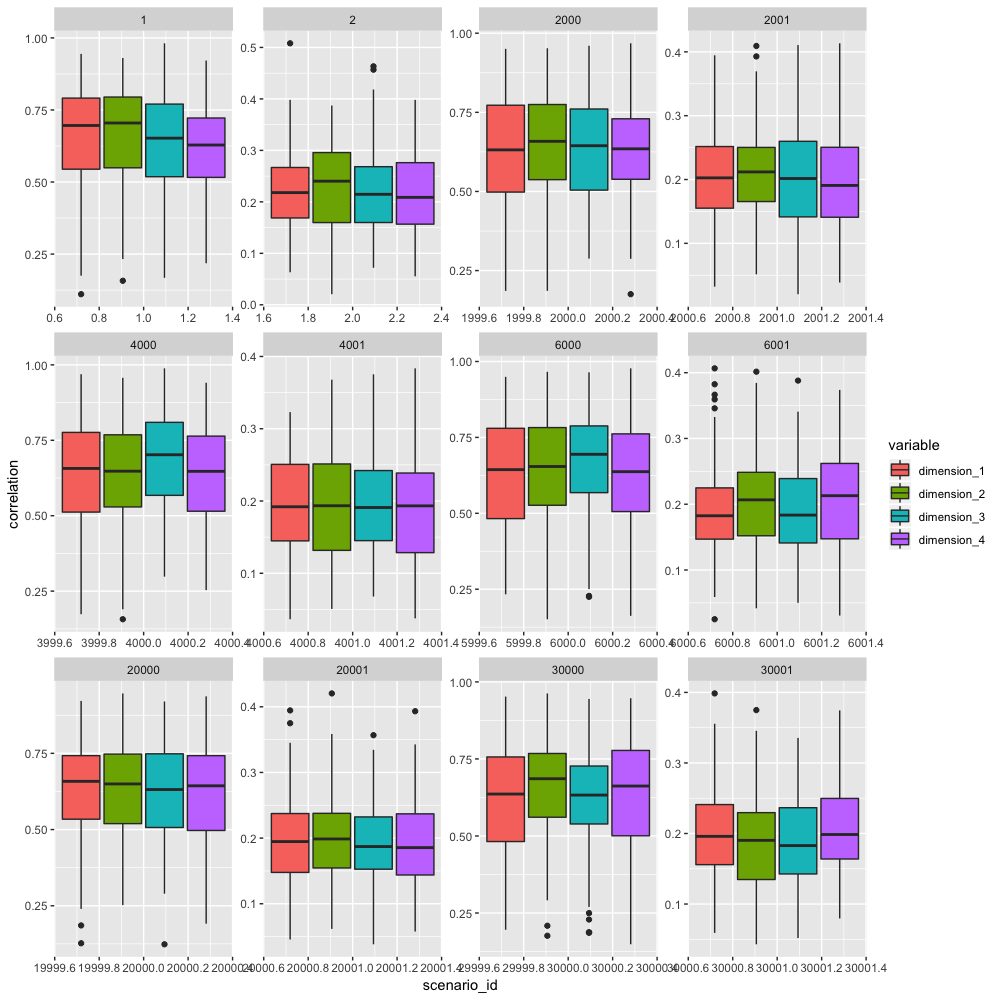
\includegraphics[width=8cm, height=10cm]{./images/gower_correlation_noise.png}
    \caption{Correlation for \textit{noisy scenarios} and MDS based on Gower algorithm.}
    \label{gower_correlation_noise}
\end{figure}


We do the same for \textit{MDS based on Gower interpolation} algorithm. 
Figure \ref{gower_correlation_1000} shows the boxplot of the correlation 
coefficients between the data and the MDS of this algorithm. Again, there is 
high correlation between them. Figure \ref{gower_correlation_noise} shows the 
boxplot for the \textit{noisy scenarios}. The remaining plots are in 
\Cref{gower_corr}.

\FloatBarrier
\section{Eigenvalues}
In this section we analyse how the eigenvalues approximate the standard 
deviation of the original variables. Given \textbf{X} $n \times k$, we say 
that the original data has $k$ variables. So, we treat the columns as 
variables. 

\indent Since the original dataset, \textbf{X}, is postmultiplied by a diagonal 
matrix $k \times k$ that contains $\lambda_1, \dots, \lambda_k$, then 
$\mbox{var}(X_i) = \lambda_i^2$ and $\mbox{sd}(X_i) = \lambda_i$. 

\indent MDS should be able to capture the variance of the main dimensions 
through the eigenvalues. Let $\phi_1, \dots, \phi_t$ be the 
\textit{normalized eigenvalues} of the MDS such that 
$\phi_1 > \phi_2 > \cdots > \phi_t$. The first highest
\textit{normalized eigenvalues} have to verify $\sqrt{\phi_j} \approx \lambda_j$.

Given a scenario, the number of main dimensions can be:

\begin{itemize}
\item 1 if there is one main dimension with $\lambda_1  = 15$.

\item 2 if there are two main dimensions with $\lambda_1  = \lambda_2 = 15$ or
with $\lambda_1  = 15$, $\lambda_2 =10$.

\item 4 if there are four main dimensions with 
$\lambda_1  = \lambda_2 = \lambda_3 = \lambda_4 = 15$.

\item 0 if it is a \textit{noisy scenario}, i.e, 
$\lambda_1  = \lambda_k = \cdots = \lambda_k = 1$.

\end{itemize}

\indent To check how the algorithms approximate the variance of the original 
data, we compute the bias and mean square error (MSE) for each scenario. We do 
not include the noisy ones. Remember that, 
$\mbox{bias} = \frac{1}{m}\sum_{i=1}^m \sqrt{\phi_{ij}} - \lambda_j = \overline{\sqrt{\phi_j}} - \lambda_j$ 
and $\mbox{MSE} = \frac{1}{m} \sum_{i = 1} ^m (\lambda_j - \sqrt{\phi_{ij}})^2$.
Since we have performed 100 simulations, $m = 100$. Depending on the scenario, 
there can be 1, 2 or 4 estimators. 

\indent Table \ref{mse_divide_one_dimensions} shows the bias and MSE for 
\textit{Divide and Conquer MDS} and scenarios with one main dimension 
$\lambda = 15$. As we can see, the bias and MSE is ``low" for these 
scenarios and this algorithm.

\indent The remaining cases are in \Cref{chap:mes}. As long as number of 
dimensions increases, the bias and MSE does the same. However, it seems to
be in an acceptable range.

\begin{table}[ht]
\centering
\begin{tabular}{rrrrr}
 & scenario\_id & $\overline{\sqrt{\phi_1}}$ & $\mbox{bias}_1$ & $\mbox{MSE}_1$ \\ 
  \hline
  1 & 3 & 14.98 & -0.02 & 0.03 \\ 
  2 & 4 & 15.03 & 0.03 & 0.11 \\ 
  3 & 2002 & 15.00 & -0.00 & 0.00 \\ 
  4 & 2003 & 14.96 & -0.04 & 0.16 \\ 
  5 & 4002 & 14.99 & -0.01 & 0.02 \\ 
  6 & 4003 & 14.99 & -0.01 & 0.01 \\ 
  7 & 6002 & 14.99 & -0.01 & 0.01 \\ 
  8 & 6003 & 14.99 & -0.01 & 0.00 \\ 
  9 & 20002 & 14.99 & -0.01 & 0.01 \\ 
  10 & 20003 & 14.99 & -0.01 & 0.01 \\ 
  11 & 30002 & 14.98 & -0.02 & 0.03 \\ 
  12 & 30003 & 14.99 & -0.01 & 0.01 \\ 
   \hline
\end{tabular}
\caption{MSE for scenarios with one main dimension $\lambda_1 = 15$ for \textit{Divide and Conquer MDS}.}
\label{mse_divide_one_dimensions}
\end{table}

\indent Table \ref{mse_fast_one_dimensions} shows the bias and MSE for 
\textit{Fast MDS} and scenarios with one main dimension $\lambda = 15$. 
There is one scenario (\textit{scenario\_id = 6002}) for which the MSE 
seems to be high. We do not know the reason, since it is one particular case. 
Apart from this scenario, the other ones 
have a small value for the bias and MSE, but a little bit higher than 
\textit{Divide and Conquer MDS}.

\indent The remaining cases are in \Cref{mse_fast}. As long as number of 
dimensions increases, the bias and MSE does the same. However, it seems to
be in an acceptable range.

\indent Table \ref{mse_gower_one_dimensions} shows the bias and the MSE for 
\textit{MDS based on Gower interpolation} and scenarios with one main 
dimension $\lambda = 15$. Again both values are small, but a little bit higher 
than \textit{Divide and Conquer MDS}.

\indent The remaining cases are in \Cref{mse_gower}. As long as number of 
dimensions increases, the bias and MSE does the same. However, it seems to
be in an acceptable range.

\indent The algorithm that has the lowest error is the 
\textit{Divide and Conquer MDS}. Even though the other ones have higher errors,
we consider that they are acceptable.

\indent Note that, we do not consider the \textit{noisy scenarios}, since all 
the directions have the same variance.


\begin{table}[ht]
\centering
\begin{tabular}{rrrrr}
 & scenario\_id & $\overline{\sqrt{\phi_1}}$ & $\mbox{bias}_1$ & $\mbox{MSE}_1$ \\
  \hline
  1 & 3 & 14.85 & -0.15 & 2.27 \\ 
  2 & 4 & 15.01 & 0.01 & 0.01 \\ 
  3 & 2002 & 14.91 & -0.09 & 0.76 \\ 
  4 & 2003 & 15.10 & 0.10 & 0.93 \\ 
  5 & 4002 & 14.96 & -0.04 & 0.14 \\ 
  6 & 4003 & 15.03 & 0.03 & 0.07 \\ 
  7 & 6002 & 14.33 & -0.67 & 44.82 \\ 
  8 & 6003 & 15.09 & 0.09 & 0.76 \\ 
  9 & 20002 & 15.00 & -0.00 & 0.00 \\ 
  10 & 20003 & 15.00 & 0.00 & 0.00 \\ 
  11 & 30002 & 14.86 & -0.14 & 1.88 \\ 
  12 & 30003 & 14.90 & -0.10 & 1.02 \\ 
   \hline
\end{tabular}
\caption{MSE for scenarios with one main dimension $\lambda_1 = 15$ for \textit{Fast MDS}.}
\label{mse_fast_one_dimensions}
\end{table}



\begin{table}[ht]
\centering
\begin{tabular}{rrrrr}
 & scenario\_id & $\overline{\sqrt{\phi_1}}$ & $\mbox{bias}_1$ & $\mbox{MSE}_1$ \\
  \hline
  1 & 3 & 15.05 & 0.05 & 0.22 \\ 
  2 & 4 & 15.02 & 0.02 & 0.04 \\ 
  3 & 2002 & 14.94 & -0.06 & 0.36 \\ 
  4 & 2003 & 15.04 & 0.04 & 0.20 \\ 
  5 & 4002 & 14.98 & -0.02 & 0.04 \\ 
  6 & 4003 & 15.02 & 0.02 & 0.05 \\ 
  7 & 6002 & 14.99 & -0.01 & 0.01 \\ 
  8 & 6003 & 15.06 & 0.06 & 0.31 \\ 
  9 & 20002 & 15.04 & 0.04 & 0.19 \\ 
  10 & 20003 & 14.97 & -0.03 & 0.07 \\ 
  11 & 30002 & 14.98 & -0.02 & 0.06 \\ 
  12 & 30003 & 14.90 & -0.10 & 1.07 \\ 
   \hline
\end{tabular}
\caption{MSE for scenarios with one main dimension $\lambda_1 = 15$ for \textit{MDS based on Gower interpolation}.}
\label{mse_gower_one_dimensions}
\end{table}



\section{Time to compute MDS}
In this section we test if there exists an algorithm that is faster than the
other ones. Our intuition is that \textit{MDS based on Gower interpolation} is
the fastest algorithm. Our intuition is based in the fact the it has the lowest
mean value, as we can see in Table \ref{mean_elapsed_time}.

\begin{table}[ht]
\centering
\begin{tabular}{rrrrrr}
 & sample\_size & n\_dimensions & mean\_divide\_conquer & mean\_fast & mean\_gower \\ 
  \hline
1 & $10^3$ & 10 & 0.27 & 0.14 & 0.10 \\ 
  2 & $10^3$ & 100 & 0.78 & 0.69 & 0.28 \\ 
  3 & $3 \cdot 10^3$ & 10 & 0.78 & 0.32 & 0.16 \\ 
  4 & $3 \cdot 10^3$ & 100 & 2.50 & 3.14 & 0.52 \\ 
  5 & $5 \cdot 10^3$ & 10 & 1.37 & 0.54 & 0.20 \\ 
  6 & $5 \cdot 10^3$ & 100 & 4.25 & 5.69 & 0.84 \\ 
  7 & $10^4$ & 10 & 2.60 & 1.81 & 0.31 \\ 
  8 & $10^4$ & 100 & 8.85 & 11.79 & 1.37 \\ 
  9 & $10^5$ & 10 & 28.10 & 11.46 & 2.44 \\ 
  10 & $10^5$ & 100 & 106.30 & 116.46 & 18.02 \\ 
  11 & $10^6$ & 10 & 420.29 & 106.59 & 53.15 \\ 
  12 & $10^6$ & 100 & 2365.46 & 1070.19 & 813.15 \\ 
   \hline
\end{tabular}
\caption{Mean of elapsed time (in seconds) to compute each algorithm.} 
\label{mean_elapsed_time}
\end{table}

\indent Table \ref{mean_elapsed_time} provides a rank between the methods: 
it seems that \textit{MDS based on Gower interpolation} is the fastest one. 
In second position it would be \textit{Fast MDS} and finally 
\textit{Divide and Conquer}.

\indent We do an hypothesis test to check it. We do an \textsf{ANOVA} test
using two factors: the sample size (which has 6 levels) and the number of 
dimensions (which has 2 levels). Instead of using the \textit{elapsed time} 
variable, we use its logarithm.

\indent Given the results of the  \textsf{ANOVA} test, which are in 
Table \ref{anova_elapsed_3_levels}, we can reject the null hypothesis. So,
there exists $\tau_{ij}$ such that $\tau_{ij} \neq 0$.   


\begin{table}[ht]
\centering
\begin{tabular}{lrrrrr}
 & Df & Sum Sq & Mean Sq & F value & Pr($>$F) \\ 
  \hline
  algorithm    & 2 & 9283.73 & 4641.86 & 32143.99 & $<2e-16$ \\ 
  sample\_size  & 5 & 108572.93 & 21714.59 & 150369.26 & $<2e-16$ \\ 
  n\_dimensions & 1 & 12868.36 & 12868.36 & 89110.86 &  $<2e-16$ \\ 
  Residuals    & 17991 & 2598.05 & 0.14 &  &  \\ 
   \hline
\end{tabular}
\caption{Results for \textsf{ANOVA} test  for differences in $\log(\mbox{elapsed\_time})$ using algorithms, sample size and  num. dimensions as factors.} 
\label{anova_elapsed_3_levels}
\end{table}

\indent We fit a linear regression with these
variables and see the magnitude of the coefficients. In addition, we plot the
distribution of $\log(\mbox{elapsed\_time})$ for all the algorithms.

\indent Table \ref{lm_all_variables} contains the value of the coefficients.
As long as either the sample size or the data dimensions increase the 
coefficients do the same (and so the time needed). Looking at the 
values for the \textit{algorithm} variable, it seems that 
\textit{MDS base on Gower interpolation} is the fastest, being the coefficient 
equal to 0. On the other hand, \textit{Divide and Conquer} is the slowest one.

\begin{table}[ht]
\centering
\begin{tabular}{rrrrr}
 & Estimate & Std. Error & t value & Pr($>$$|$t$|$) \\ 
  \hline
(Intercept) & -1.4058 & 0.0085 & -165.44 & $<2e-16$ \\ 
  algorithmfast & -0.4313 & 0.0069 & -62.17 & $<2e-16$ \\ 
  algorithmgower & -1.6926 & 0.0069 & -243.96 & $<2e-16$ \\ 
  sample\_size3000 & 0.9473 & 0.0098 & 96.54 & $<2e-16$ \\ 
  sample\_size5000 & 1.4434 & 0.0098 & 147.10 & $<2e-16$ \\ 
  sample\_size10000 & 2.1505 & 0.0098 & 219.17 & $<2e-16$ \\ 
  sample\_size1e+05 & 4.4286 & 0.0098 & 451.35 & $<2e-16$ \\ 
  sample\_size1e+06 & 7.2782 & 0.0098 & 741.78 & $<2e-16$ \\ 
  n\_dimensions100 & 1.6910 & 0.0057 & 298.51 & $<2e-16$ \\ 
   \hline
\end{tabular}
\caption{Linear model for response $\log(\mbox{elapsed\_time})$.} 
\label{lm_all_variables}
\end{table}

\indent Figure \ref{elapsed_time_1000} shows the estimated density of the
elapsed time for each algorithm and each \textit{scenario\_id}. As we can see, 
\textit{MDS based on Gower interpolation} is the fastest algorithm, especially
when 100 dimensions are required. Figure \ref{elapsed_time_1000} contains the 
\textit{scenario\_id}'s just for the sample size $n = 10^3$. The remaining 
figures are in \Cref{elapsed_time_alg}. One interesting thing that we can
observe from \Cref{elapsed_time_alg} is the fact that the elapsed time grows
as long as the sample size does, especially form \textit{Divide and Conquer MDS}.
However, \textit{MDS based on Gower interpolation} and \textit{Fast MDS} 
provide a really good time even though the sample size is big, being
\textit{MDS based on Gower interpolation} the fastest one. So, we can consider
both algorithms efficient, since they are able to compute MDS is a reasonable
amount of time.


\begin{figure}[!ht]
\centering
    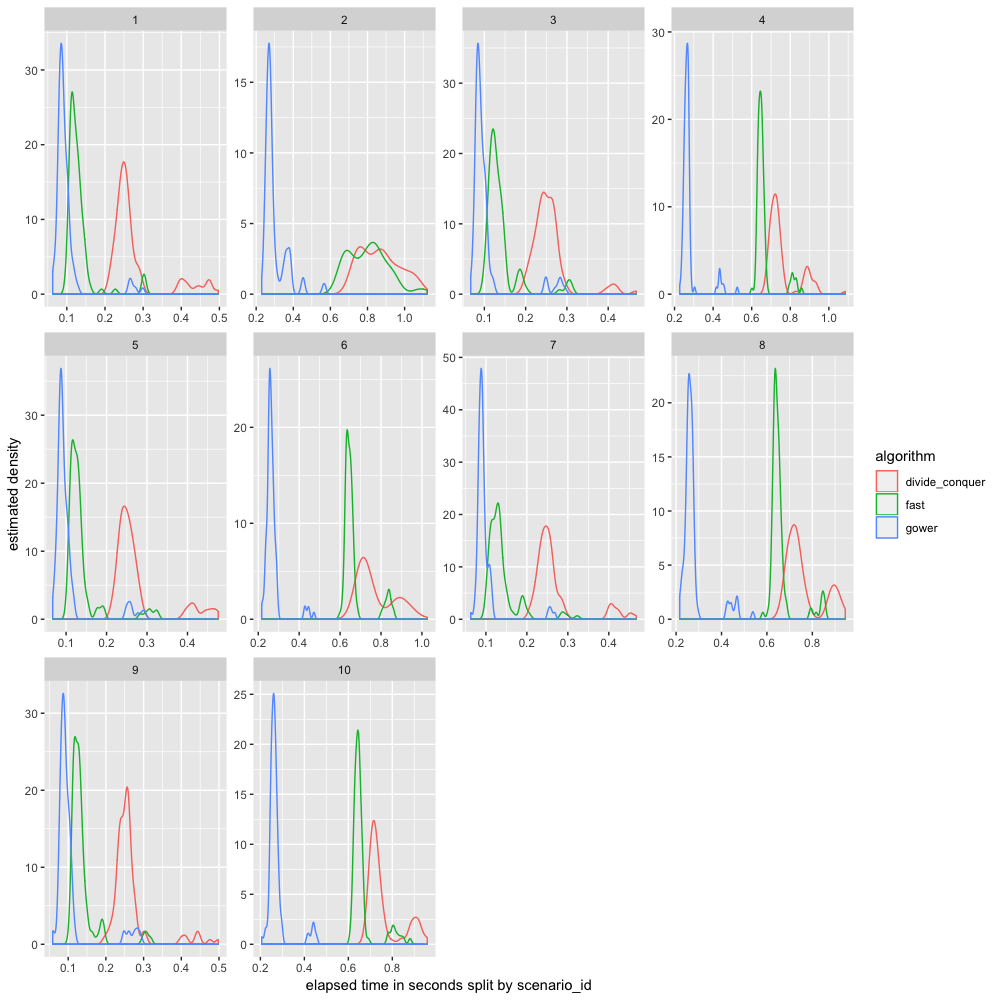
\includegraphics{./images/elapsed_time_1000.png}
    \caption{Elapsed time for each algorithm and each \textit{scenario\_id} of $n=10^3$.}
    \label{elapsed_time_1000}
\end{figure}


\indent After seeing the estimated density, we would like to test if there 
exists any difference between the scenarios To test that, we perform, again, an 
\textsf{ANOVA} test. This test includes two factors: \textit{scenario\_id},
which has 60 levels, and algorithms, which has 3 levels. As a response, we use
the logarithm of the elapsed time.

\indent Table \ref{anova_elapsed_all_scenarios} contains the result for the 
hypothesis test. We can reject the null hypothesis, at least one level is 
different from the other ones in terms of elapsed time.

\begin{table}[ht]
\centering
\begin{tabular}{lrrrrr}
 & Df & Sum Sq & Mean Sq & F value & Pr($>$F) \\ 
  \hline
scenario\_id & 59 & 121912.97 & 2066.32 & 17431.46 & $<2e-16$ \\ 
  algorithm   & 2 & 9283.73 & 4641.86 & 39158.68 & $<2e-16$ \\ 
  Residuals   & 17938 & 2126.37 & 0.12 &  &  \\ 
   \hline
\end{tabular}
\caption{Results for \textsf{ANOVA} test  for differences in $\log(\mbox{elapsed\_time})$ using \textit{scenario\_id} and algorithms as factors.} 
\label{anova_elapsed_all_scenarios}
\end{table}



\chapter{Conclusions}
The goal of this master's thesis was to find an algorithm able to compute a MDS
configuration when dealing with a big dataset in an ``efficient" way, i.e, 
such an algorithm should be fast enough to get the configuration.

\indent The first algorithm developed, \textit{Divide and Conquer MDS}, does not 
achieve the goal. Although we have managed to get a MDS configuration, too much 
time is required. However, it has a really good property 
that the other two algorithms do not have: it is able to capture the variance
of the original data quite well. 

\indent Even though \textit{Fast MDS} solves the problem of time, it is based on 
recursive programming. The problem with these kind of algorithms is that they
can consume a lot of memory. 

\indent A really good algorithm is \textit{MDS based on Gower interpolation},
since it provides a MDS configuration in small amount of time with low errors 
and its implementation is easy. Apart from this, it does not need to do 
any Procrustes transformation, which save time and memory. Therefore, this 
would be the algorithm to use if MDS had to be computed with large datasets.\\


\noindent{\textbf{Problem encountered during the development of the thesis}}

\indent Basically we have faced two kind of problems, which are:

\begin{itemize}
\item Computational problems: when working with big datasets, we suffered from
consuming all RAM of the servers. Especially when doing Procrustes for aligning
the original data and the MDS for $n$ large. The solution to it was to partition
the process into pieces that the servers could manage without consuming all RAM.

\item Procrustes packages: even though \textsf{R} has a lot of packages that
allows to compute Procrustes, they did not fulfilled our goals. The reasons are
either because the output is not well specified or because some of the 
transformations (mainly dilations or translations) were not included. We 
recommend to use \textsf{MCMCpack} package.

\end{itemize}

\noindent{\textbf{Future research}}

\indent The algorithms that we have developed are implemented in \textsf{R},
which is a good language to do prototypes. However, this is not the best
programming language to be used. So, we recommend to implement them in a robust 
programming language such as \textsf{C}, \textsf{C++} or \textsf{Java}.

\indent Given that the world is talking about Big Data, it is a good 
opportunity to challenge the algorithms and use them with Spark/Hadoop. Actually
the initial idea of this thesis was to use them with a Spark DB that contains
millions of chess games. Due to lack of time, we could not do so. \\


\noindent{\textbf{Acknowledgements}}

I would like to express my gratitude to \textit{Pedro Delicado}, since he helped
me to do this thesis. There have been some difficult issues in which his help
allowed me to move on and solve them. Also, I would like to thank
\textit{Roger Devesa}, since he has helped me with reviewing recursive 
programming and with implementing \textit{Fast MDS}.



\bibliographystyle{chicago}
\bibliography{bibliography.bib}


\appendix 

\chapter{Correlation coefficients boxplot}

\section{Divide and Conquer MDS}
\label{div_conquer_corr}

\begin{figure}[ht]
\centering
    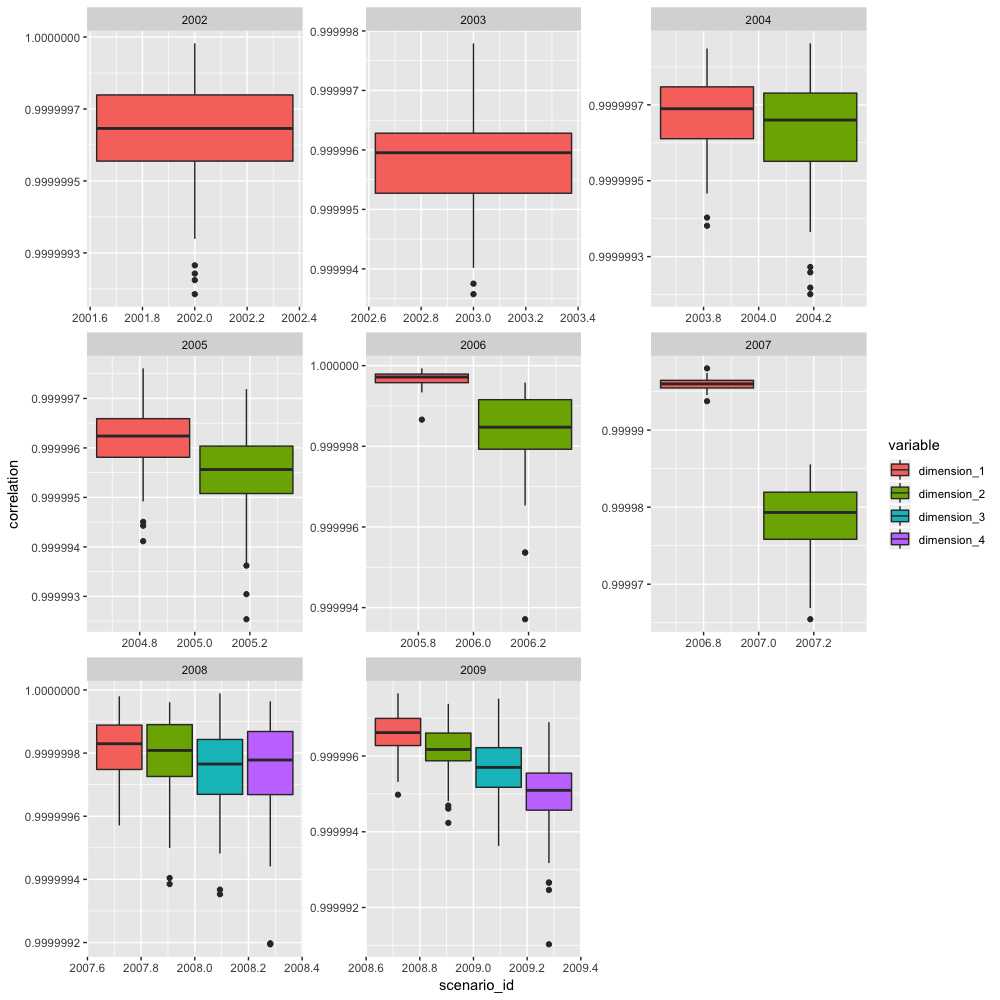
\includegraphics[scale = 1.5]{./images/divide_correlation_3000.png}
    \caption{Correlation for $n = 3 \cdot 10^3$ and MDS Divide and conquer algorithm}
    \label{divide_correlation_3000}
\end{figure}

\begin{figure}[ht]
\centering
    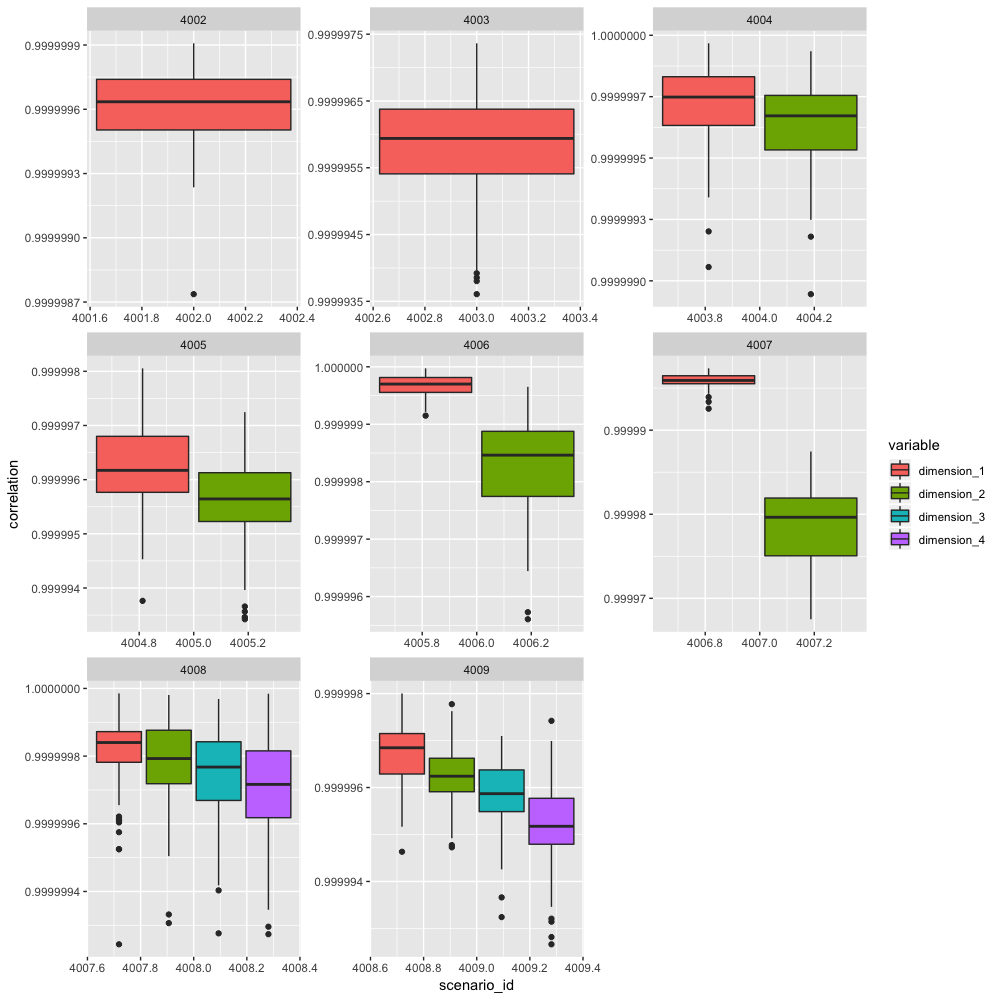
\includegraphics[scale = 1.5]{./images/divide_correlation_5000.png}
    \caption{Correlation for $n = 5 \cdot 10^3$ and MDS Divide and conquer algorithm}
    \label{divide_correlation_5000}
\end{figure}

\begin{figure}[ht]
\centering
    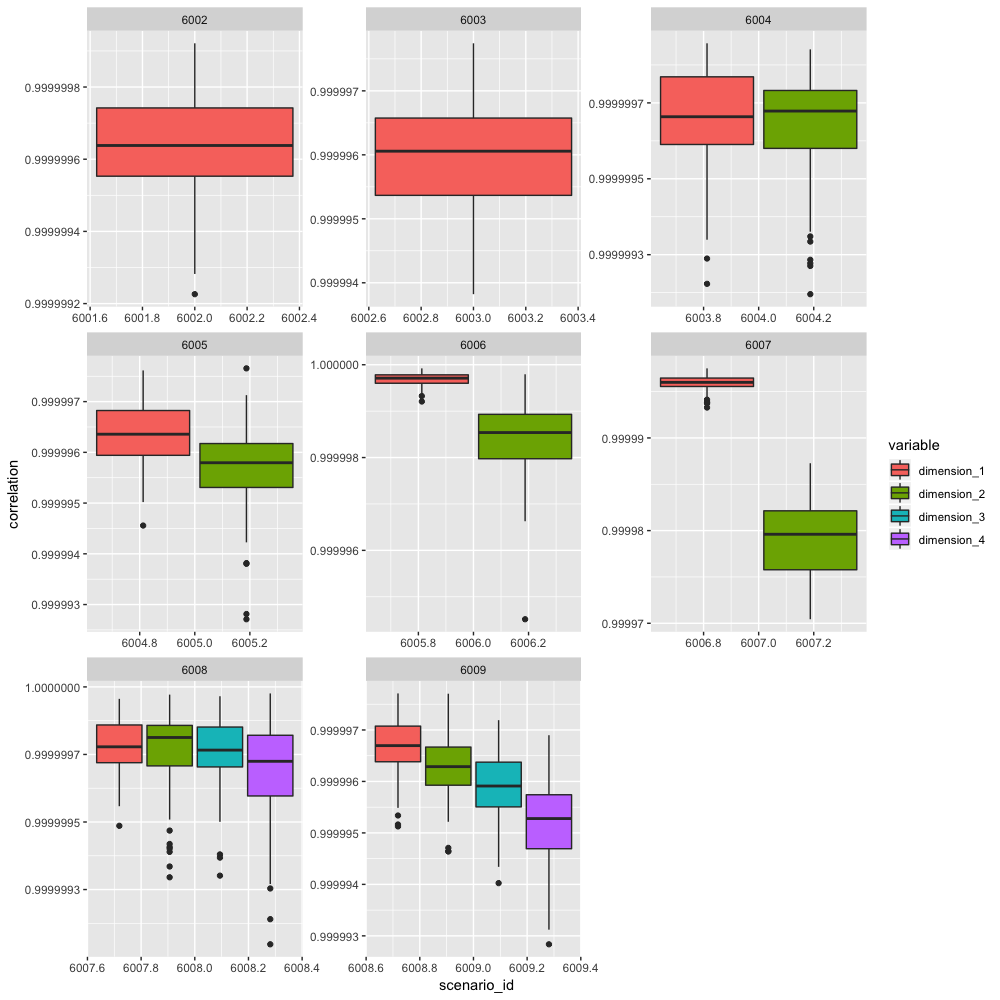
\includegraphics[scale = 1.5]{./images/divide_correlation_10000.png}
    \caption{Correlation for $n = 10^4$ and MDS Divide and conquer algorithm}
    \label{divide_correlation_10000}
\end{figure}

\begin{figure}[ht]
\centering
    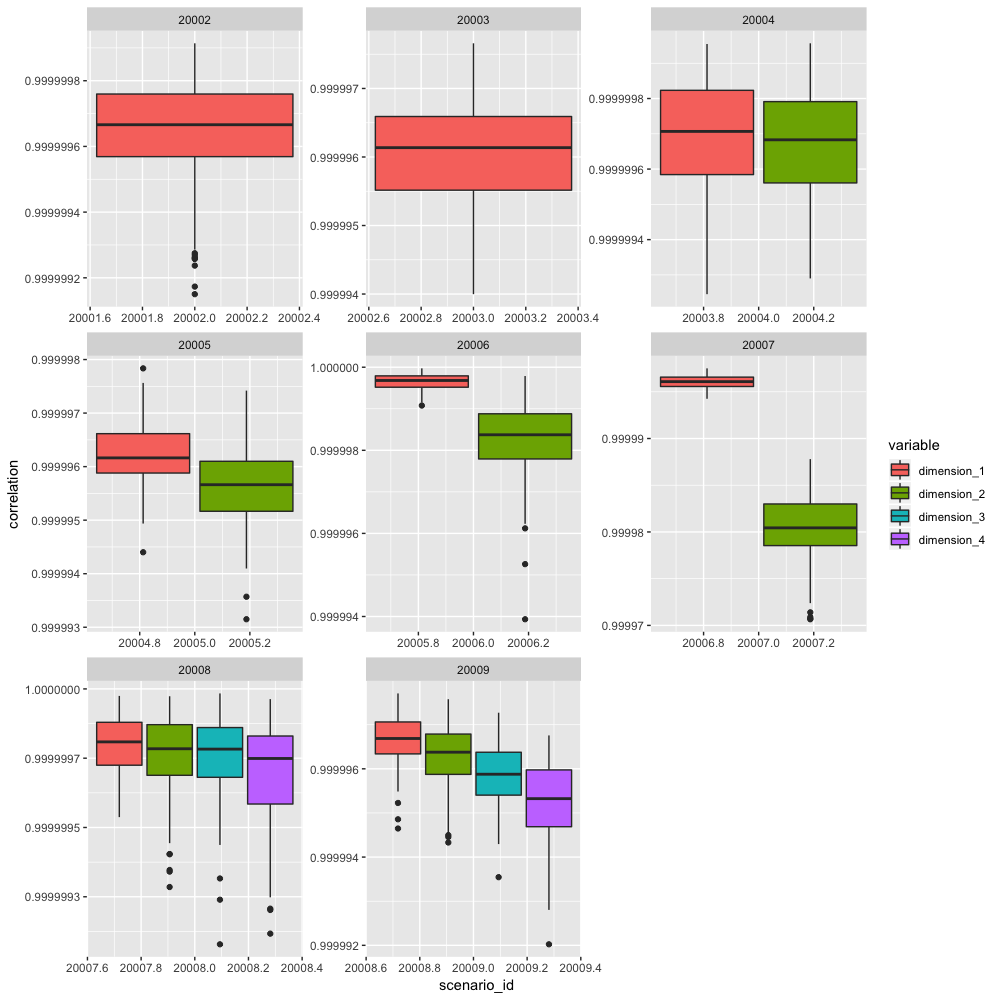
\includegraphics[scale = 1.5]{./images/divide_correlation_100000.png}
    \caption{Correlation for $n = 10^5$ and MDS Divide and conquer algorithm}
    \label{divide_correlation_100000}
\end{figure}

\begin{figure}[ht]
\centering
    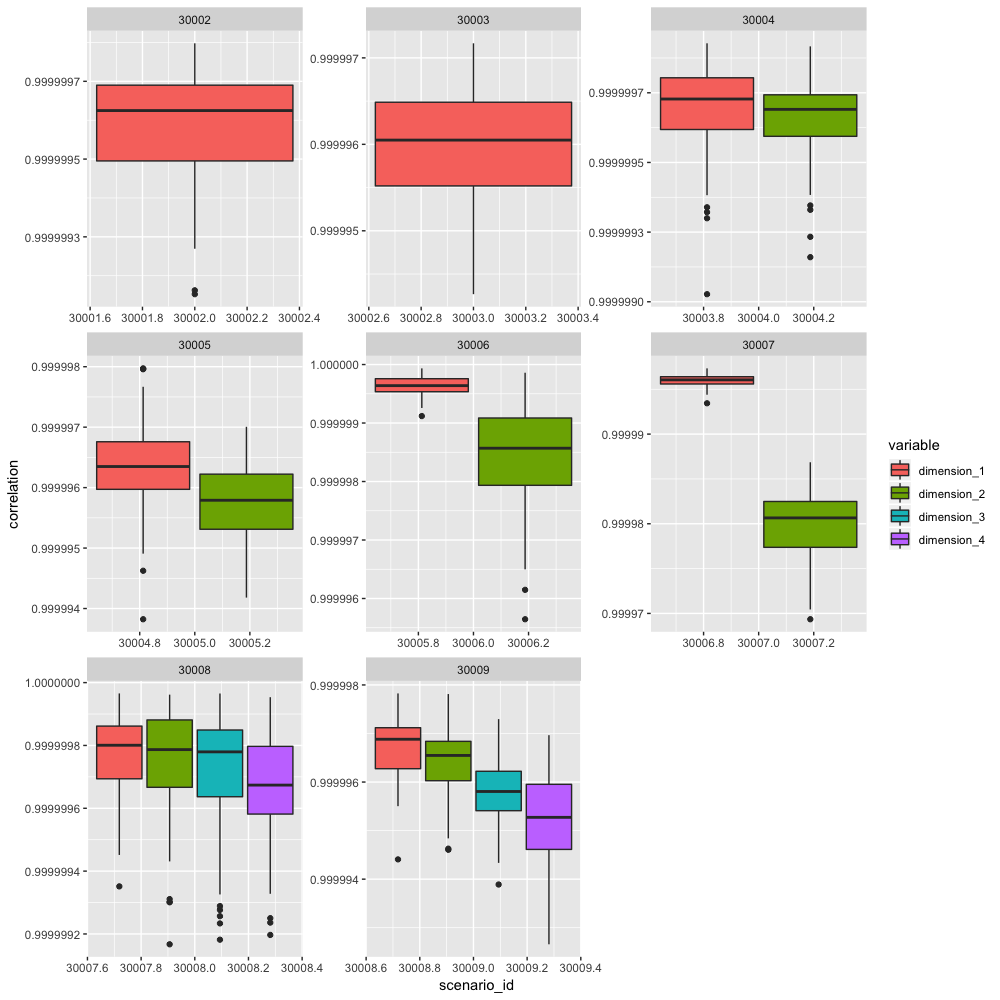
\includegraphics[scale = 1.5]{./images/divide_correlation_1000000.png}
    \caption{Correlation for $n = 10^6$ and MDS Divide and conquer algorithm}
    \label{divide_correlation_1000000}
\end{figure}
\FloatBarrier

\section{Fast MDS}
\label{fast_corr}
\begin{figure}[ht]
\centering
    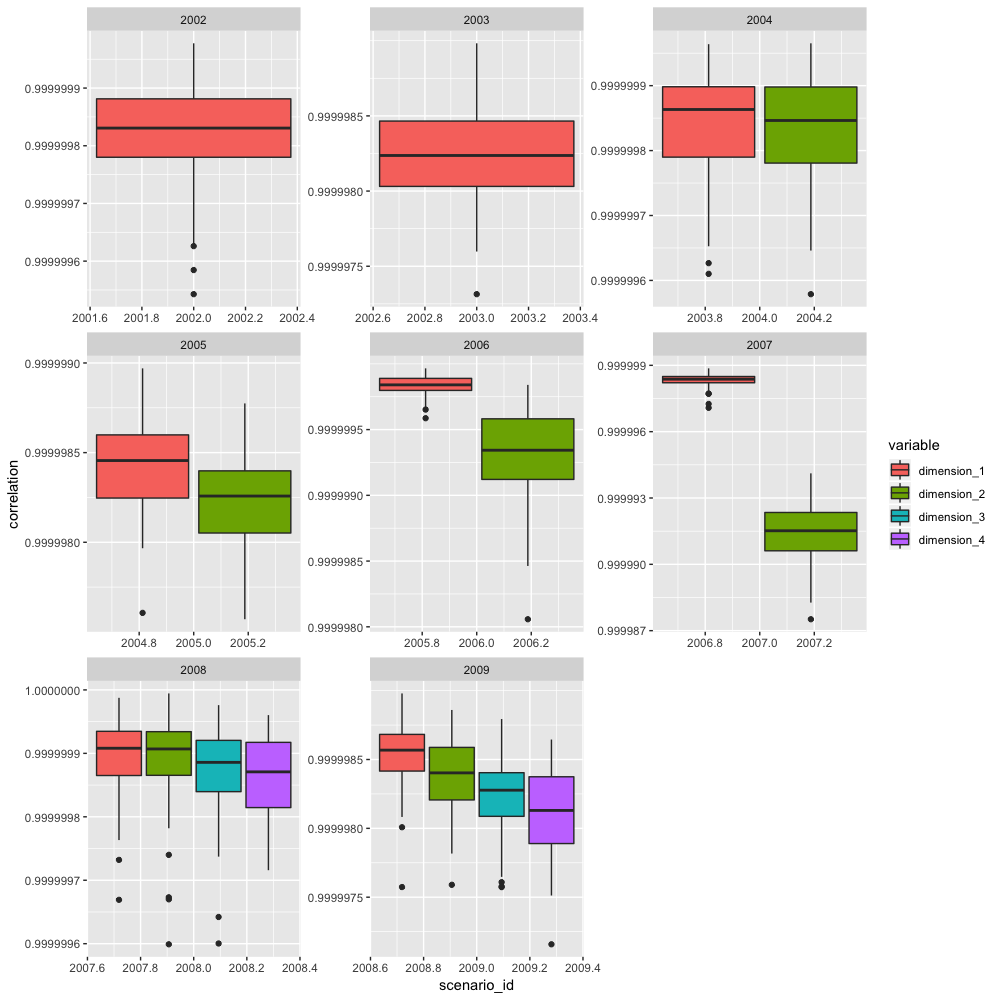
\includegraphics[scale = 1.5]{./images/fast_correlation_3000.png}
    \caption{Correlation for $n = 3 \cdot 10^3$ and MDS Fast algorithm.}
    \label{fast_correlation_3000}
\end{figure}

\begin{figure}[ht]
\centering
    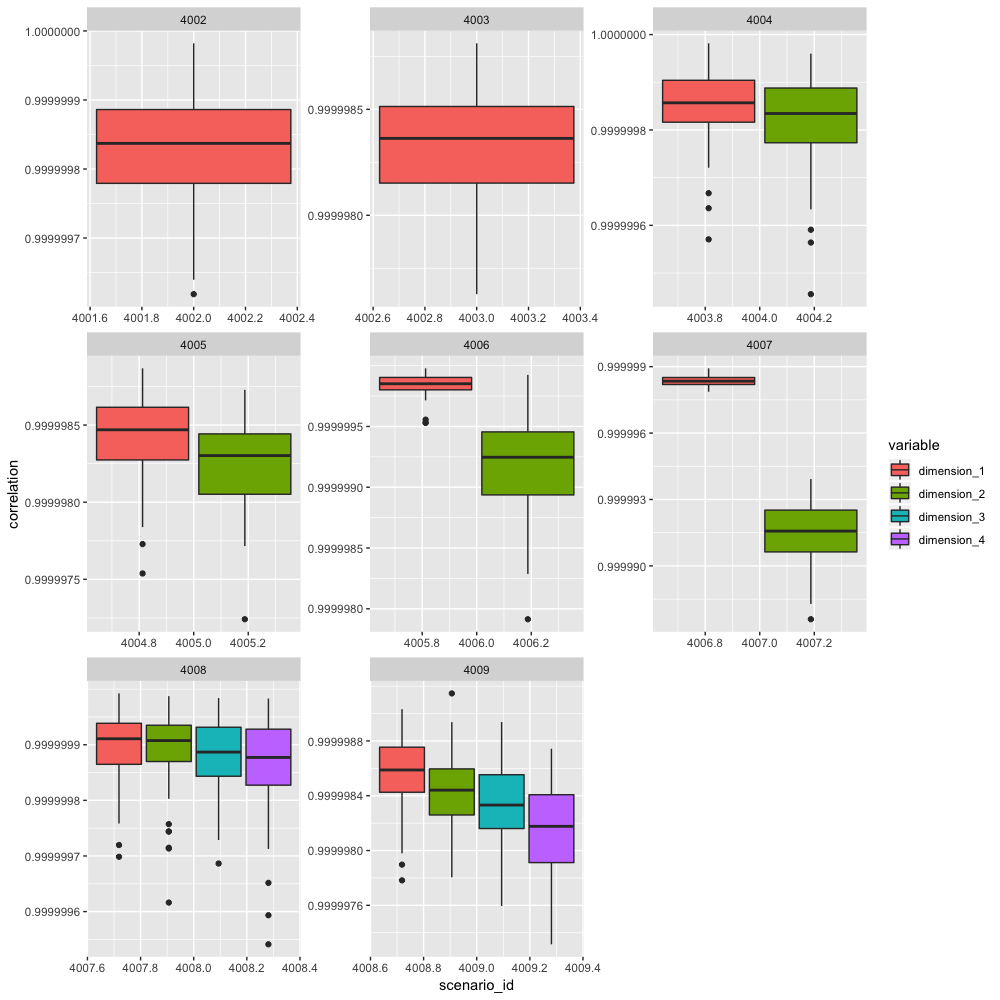
\includegraphics[scale = 1.5]{./images/fast_correlation_5000.png}
    \caption{Correlation for $n = 5 \cdot 10^3$ and MDS Fast algorithm.}
    \label{fast_correlation_5000}
\end{figure}

\begin{figure}[ht]
\centering
    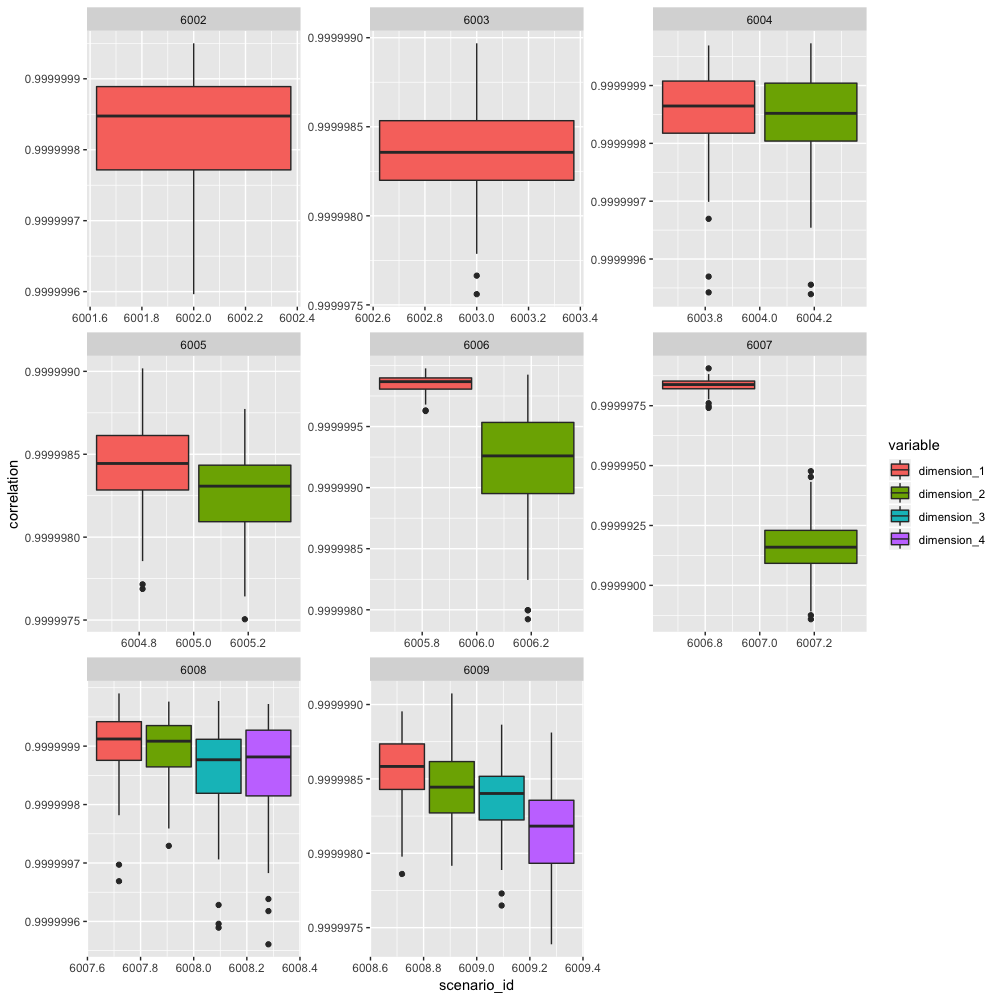
\includegraphics[scale = 1.5]{./images/fast_correlation_10000.png}
    \caption{Correlation for $n = 10^4$ and MDS Fast algorithm.}
    \label{fast_correlation_10000}
\end{figure}

\begin{figure}[ht]
\centering
    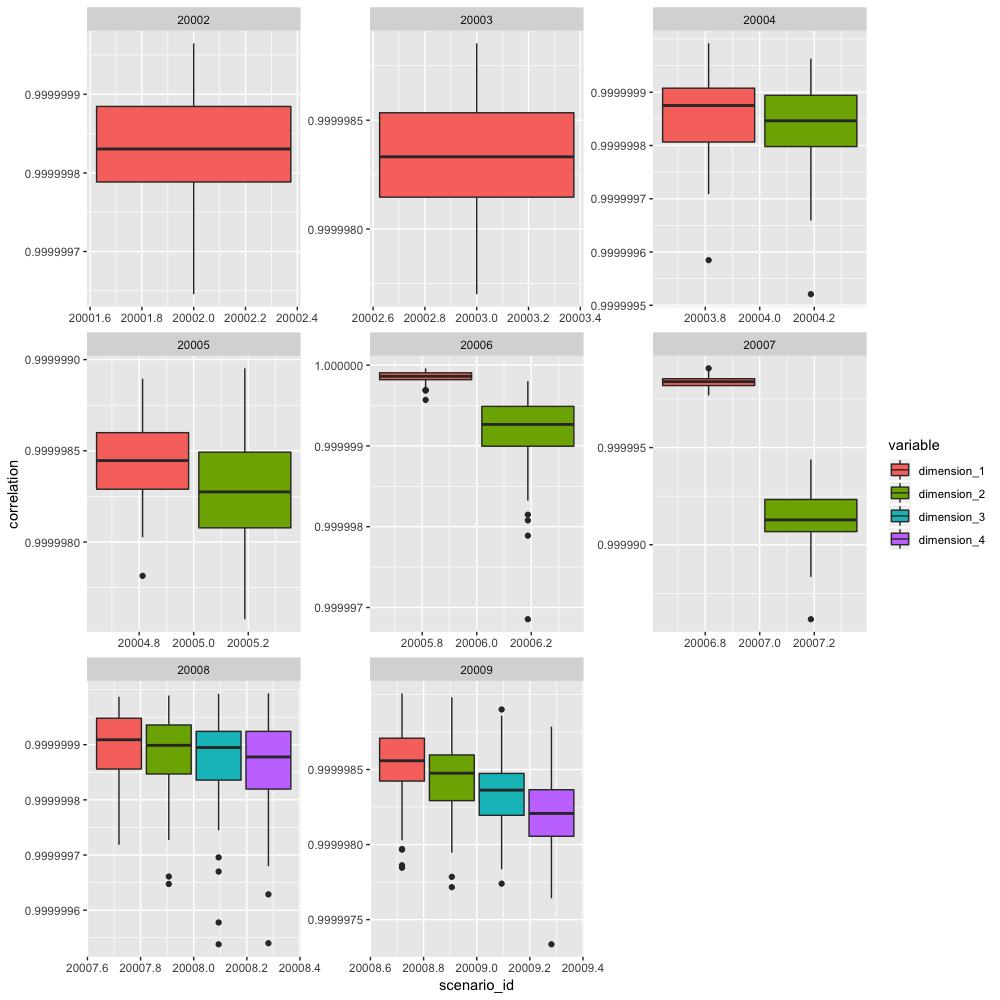
\includegraphics[scale = 1.5]{./images/fast_correlation_100000.png}
    \caption{Correlation for $n = 10^5$ and MDS Fast algorithm.}
    \label{fast_correlation_100000}
\end{figure}

\begin{figure}[ht]
\centering
    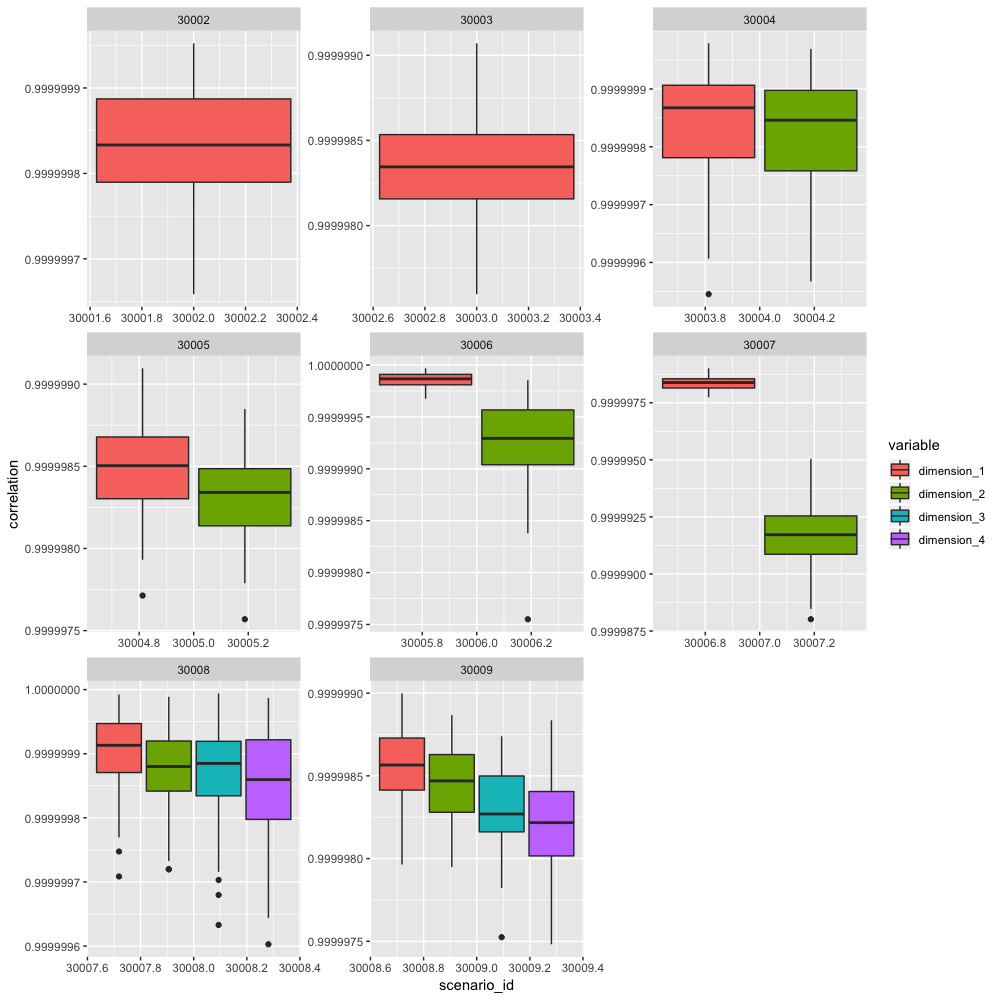
\includegraphics[scale = 1.5]{./images/fast_correlation_1000000.png}
    \caption{Correlation for $n = 10^6$ and MDS Fast algorithm.}
    \label{fast_correlation_1000000}
\end{figure}

\FloatBarrier

\section{MDS based on Gower interpolation}
\label{gower_corr}

\begin{figure}[ht]
\centering
    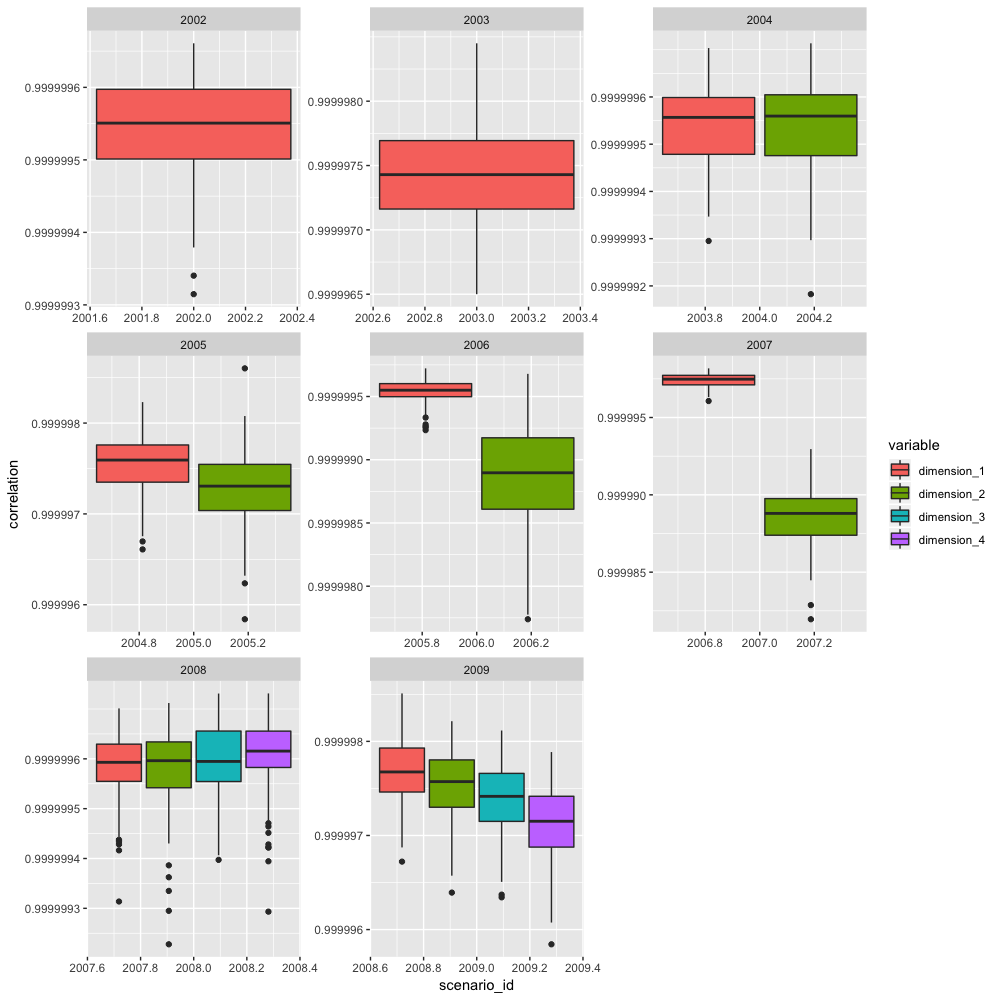
\includegraphics[scale = 1.5]{./images/gower_correlation_3000.png}
    \caption{Correlation for $n = 3 \cdot 10^3$ and MDS based on Gower interpolation algorithm.}
    \label{gower_correlation_3000}
\end{figure}

\begin{figure}[ht]
\centering
    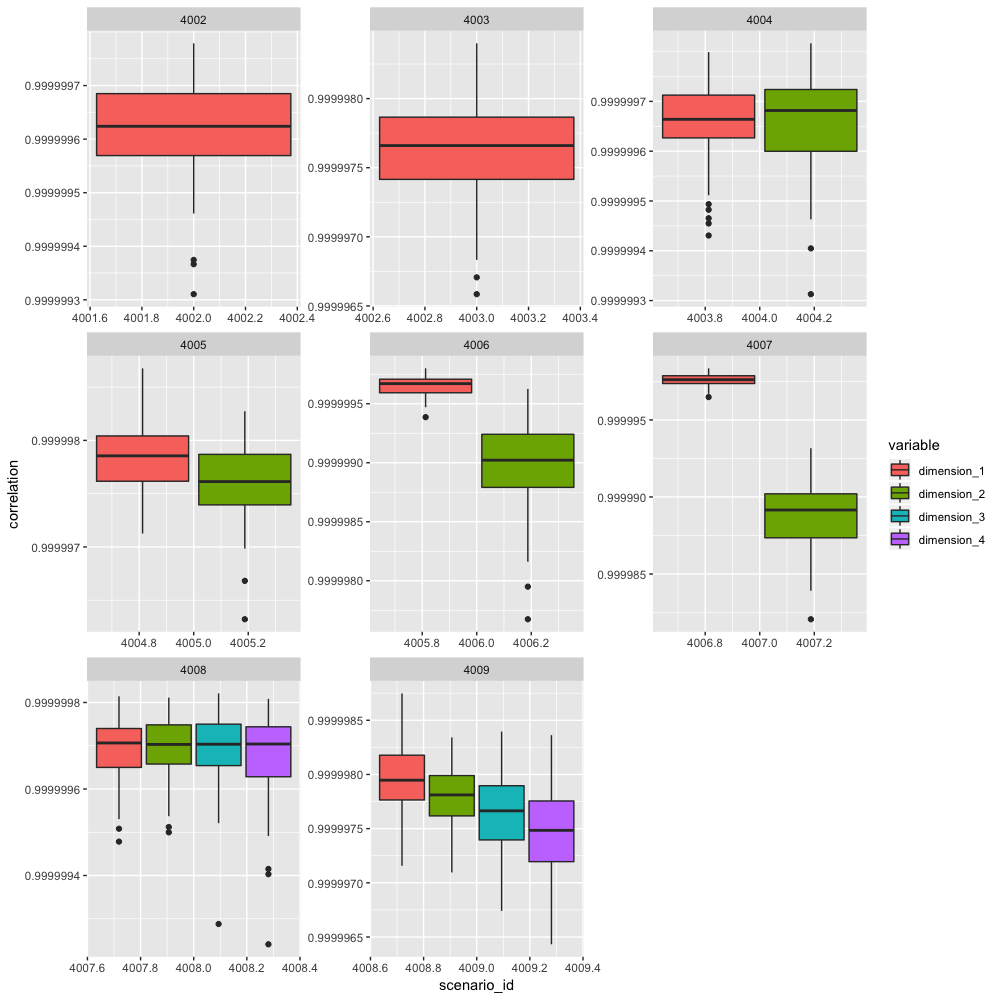
\includegraphics[scale = 1.5]{./images/gower_correlation_5000.png}
    \caption{Correlation for $n = 5 \cdot 10^3$ and MDS based on Gower interpolation algorithm.}
    \label{gower_correlation_5000}
\end{figure}

\begin{figure}[ht]
\centering
    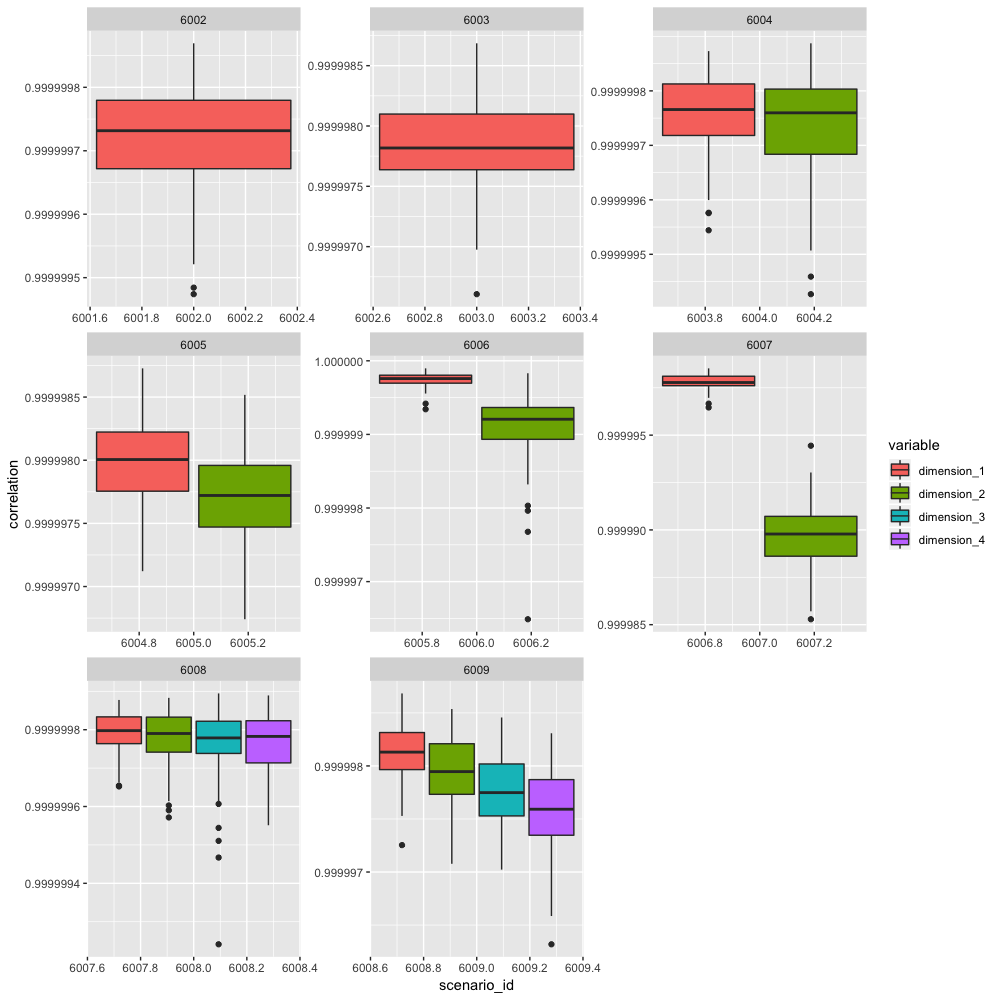
\includegraphics[scale = 1.5]{./images/gower_correlation_10000.png}
    \caption{Correlation for $n = 10^4$ and MDS based on Gower interpolation algorithm.}
    \label{gower_correlation_10000}
\end{figure}

\begin{figure}[ht]
\centering
    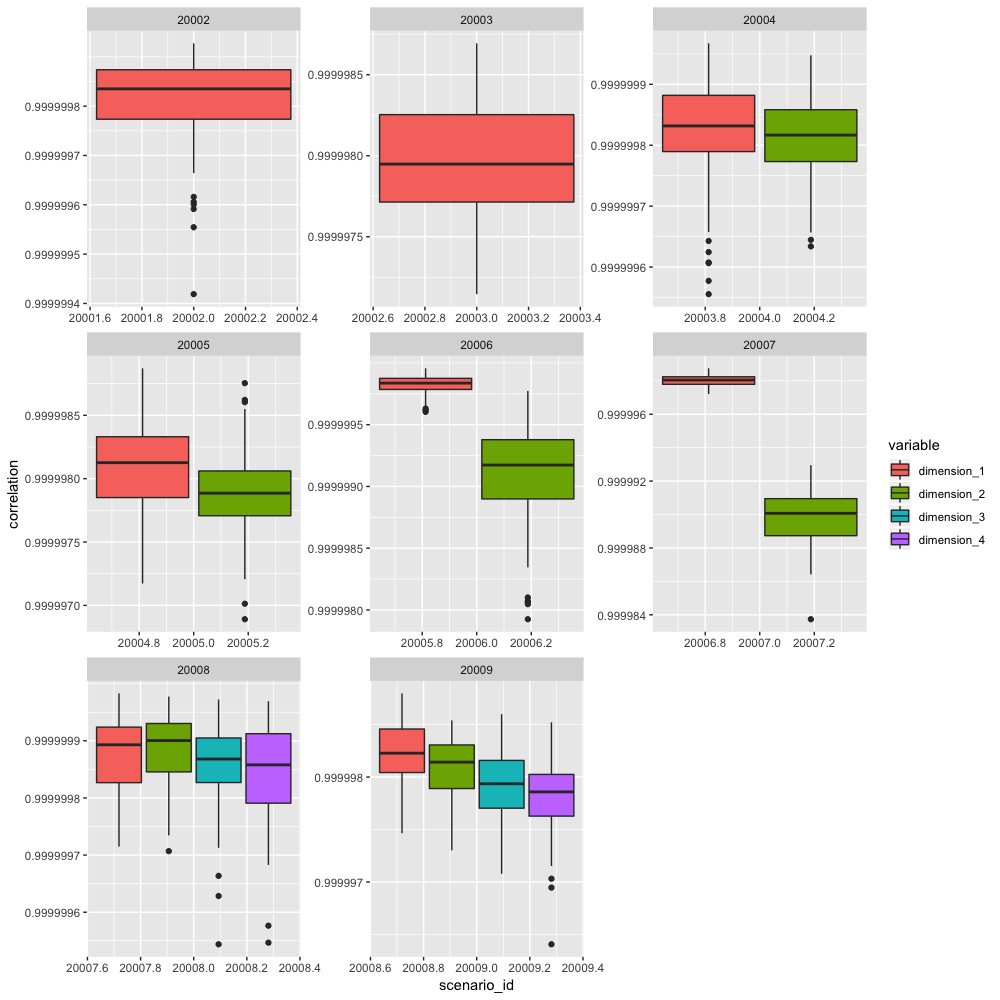
\includegraphics[scale = 1.5]{./images/gower_correlation_100000.png}
    \caption{Correlation for $n = 10^5$ and MDS based on Gower interpolation algorithm.}
    \label{gower_correlation_100000}
\end{figure}

\begin{figure}[ht]
\centering
    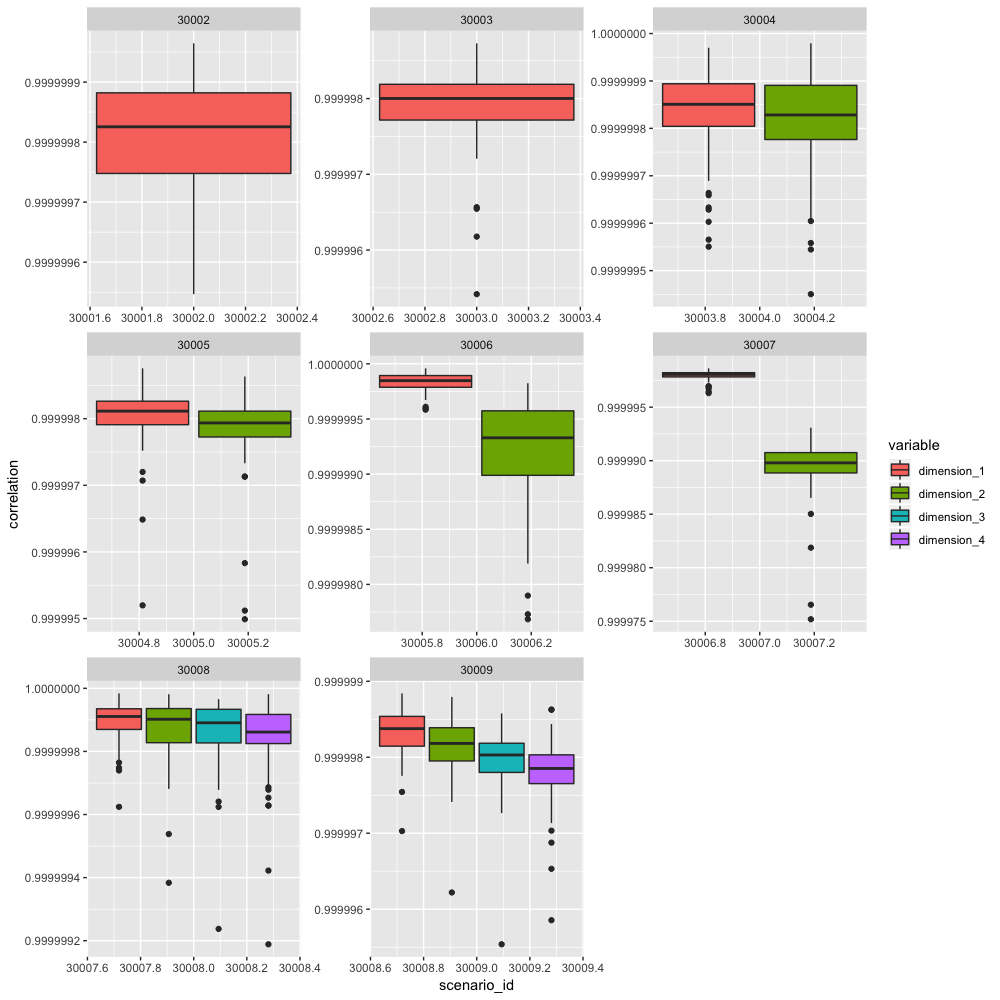
\includegraphics[scale = 1.5]{./images/gower_correlation_1000000.png}
    \caption{Correlation for $n = 10^6$ and MDS based on Gower interpolation algorithm.}
    \label{gower_correlation_1000000}
\end{figure}


\chapter{Bias and MSE for eigenvalues}
\section{Divide and Conquer MDS}
\label{chap:mes}

\begin{table}[ht]
\centering
\begin{tabular}{rrrrrrrr}
 & scenario\_id & $\overline{\sqrt{\phi_1}}$ & $\mbox{bias}_1$ & $\mbox{MSE}_1$ & $\overline{\sqrt{\phi_2}}$ & $\mbox{bias}_2$ & $\mbox{MSE}_2$ \\ 
  \hline
  1 & 5 & 15.41 & 0.41 & 17.12 & 14.59 & 0.41 & 16.99 \\ 
  2 & 6 & 15.41 & 0.41 & 17.08 & 14.54 & 0.41 & 20.88 \\ 
  3 & 2004 & 15.40 & 0.40 & 15.99 & 14.55 & 0.40 & 19.89 \\ 
  4 & 2005 & 15.39 & 0.39 & 15.03 & 14.54 & 0.39 & 21.59 \\ 
  5 & 4004 & 15.41 & 0.41 & 16.71 & 14.55 & 0.41 & 20.01 \\ 
  6 & 4005 & 15.41 & 0.41 & 16.94 & 14.57 & 0.41 & 18.79 \\ 
  7 & 6004 & 15.39 & 0.39 & 15.57 & 14.54 & 0.39 & 21.13 \\ 
  8 & 6005 & 15.42 & 0.42 & 17.60 & 14.57 & 0.42 & 18.22 \\ 
  9 & 20004 & 15.40 & 0.40 & 15.77 & 14.56 & 0.40 & 19.42 \\ 
  10 & 20005 & 15.41 & 0.41 & 16.85 & 14.56 & 0.41 & 19.15 \\ 
  11 & 30004 & 15.40 & 0.40 & 16.00 & 14.56 & 0.40 & 19.52 \\ 
  12 & 30005 & 15.41 & 0.41 & 16.73 & 14.56 & 0.41 & 18.96 \\ 
   \hline
\end{tabular}
\caption{Estimator, bias and MSE for scenarios with two main dimensions $\lambda_1 = 15$ and $\lambda_2 = 15$ for \textit{Divide and Conquer MDS}.}
\end{table}

\begin{table}[ht]
\centering
\begin{tabular}{rrrrrrrr}
 & scenario\_id & $\overline{\sqrt{\phi_1}}$ & $\mbox{bias}_1$ & $\mbox{MSE}_1$ & $\overline{\sqrt{\phi_2}}$ & $\mbox{bias}_2$ & $\mbox{MSE}_2$ \\ 
  \hline
  1 & 7 & 14.96 & -0.04 & 0.15 & 9.95 & -0.05 & 0.27 \\ 
  2 & 8 & 14.98 & -0.02 & 0.02 & 9.92 & -0.08 & 0.57 \\ 
  3 & 2006 & 15.01 & 0.01 & 0.02 & 9.98 & -0.02 & 0.05 \\ 
  4 & 2007 & 15.03 & 0.03 & 0.08 & 9.98 & -0.02 & 0.04 \\ 
  5 & 4006 & 15.00 & 0.00 & 0.00 & 9.99 & -0.01 & 0.02 \\ 
  6 & 4007 & 15.01 & 0.01 & 0.01 & 9.97 & -0.03 & 0.11 \\ 
  7 & 6006 & 15.01 & 0.01 & 0.01 & 9.97 & -0.03 & 0.06 \\ 
  8 & 6007 & 15.01 & 0.01 & 0.00 & 10.00 & -0.00 & 0.00 \\ 
  9 & 20006 & 15.00 & 0.00 & 0.00 & 9.98 & -0.02 & 0.05 \\ 
  10 & 20007 & 15.01 & 0.01 & 0.00 & 9.98 & -0.02 & 0.04 \\ 
  11 & 30006 & 15.00 & -0.00 & 0.00 & 9.97 & -0.03 & 0.08 \\ 
  12 & 30007 & 15.00 & 0.00 & 0.00 & 9.98 & -0.02 & 0.03 \\ 
   \hline
\end{tabular}
\caption{Estimator, bias and MSE for scenarios with two main dimensions $\lambda_1 = 15$ and $\lambda_2 = 10$ for \textit{Divide and Conquer MDS}.}
\end{table}

\begin{table}[ht]
\centering
\resizebox{\textwidth}{!}{\begin{tabular}{rrrrrrrrrrrrrr}
& scenario\_id & $\overline{\sqrt{\phi_1}}$ & $\mbox{bias}_1$ & $\mbox{MSE}_1$ & $\overline{\sqrt{\phi_2}}$ & $\mbox{bias}_2$ & $\mbox{MSE}_2$ & $\overline{\sqrt{\phi_3}}$ & $\mbox{bias}_3$ & $\mbox{MSE}_3$ & $\overline{\sqrt{\phi_4}}$ & $\mbox{bias}_4$ & $\mbox{MSE}_4$\\   
  \hline
  1 & 9 & 15.88 & 0.88 & 77.09 & 15.26 & 0.26 & 6.94 & 14.71 & -0.29 & 8.40 & 14.08 & -0.92 & 84.94 \\ 
  2 & 10 & 15.89 & 0.89 & 80.08 & 15.26 & 0.26 & 6.52 & 14.70 & -0.30 & 8.82 & 14.09 & -0.91 & 83.59 \\ 
  3 & 2008 & 15.90 & 0.90 & 80.98 & 15.26 & 0.26 & 6.87 & 14.68 & -0.32 & 10.37 & 14.04 & -0.96 & 91.72 \\ 
  4 & 2009 & 15.88 & 0.88 & 76.61 & 15.25 & 0.25 & 6.02 & 14.70 & -0.30 & 9.07 & 14.04 & -0.96 & 91.55 \\ 
  5 & 4008 & 15.87 & 0.87 & 76.05 & 15.26 & 0.26 & 6.58 & 14.68 & -0.32 & 9.99 & 14.06 & -0.94 & 87.55 \\ 
  6 & 4009 & 15.87 & 0.87 & 75.86 & 15.24 & 0.24 & 5.83 & 14.68 & -0.32 & 10.21 & 14.07 & -0.93 & 86.76 \\ 
  7 & 6008 & 15.89 & 0.89 & 79.01 & 15.25 & 0.25 & 6.07 & 14.69 & -0.31 & 9.80 & 14.06 & -0.94 & 87.95 \\ 
  8 & 6009 & 15.91 & 0.91 & 82.54 & 15.25 & 0.25 & 6.32 & 14.69 & -0.31 & 9.64 & 14.06 & -0.94 & 87.92 \\ 
  9 & 20008 & 15.89 & 0.89 & 78.58 & 15.25 & 0.25 & 6.10 & 14.68 & -0.32 & 9.98 & 14.06 & -0.94 & 87.77 \\ 
  10 & 20009 & 15.89 & 0.89 & 79.78 & 15.25 & 0.25 & 6.30 & 14.69 & -0.31 & 9.69 & 14.07 & -0.93 & 86.87 \\ 
  11 & 30008 & 15.89 & 0.89 & 78.65 & 15.25 & 0.25 & 6.09 & 14.68 & -0.32 & 9.95 & 14.06 & -0.94 & 88.05 \\ 
  12 & 30009 & 15.89 & 0.89 & 79.73 & 15.25 & 0.25 & 6.40 & 14.69 & -0.31 & 9.57 & 14.07 & -0.93 & 86.68 \\ 
   \hline
\end{tabular}}
\caption{Estimator, bias and MSE for scenarios with four main dimensions $\lambda_i = 15$ $i \in \{1,2,3,4\}$ for \textit{Divide and Conquer MDS}.}
\end{table}

\FloatBarrier


\section{Fast MDS}
\label{mse_fast}
\begin{table}[ht]
\centering
\begin{tabular}{rrrrrrrr}
 & scenario\_id & $\overline{\sqrt{\phi_1}}$ & $\mbox{bias}_1$ & $\mbox{MSE}_1$ & $\overline{\sqrt{\phi_2}}$ & $\mbox{bias}_2$ & $\mbox{MSE}_2$ \\ 
  \hline
  1 & 5 & 16.06 & 1.06 & 112.12 & 13.79 & -1.21 & 145.86 \\ 
  2 & 6 & 15.41 & 0.41 & 17.21 & 14.56 & -0.44 & 19.44 \\ 
  3 & 2004 & 15.71 & 0.71 & 49.84 & 14.31 & -0.69 & 46.93 \\ 
  4 & 2005 & 15.40 & 0.40 & 15.93 & 14.39 & -0.61 & 37.06 \\ 
  5 & 4004 & 15.50 & 0.50 & 24.80 & 14.43 & -0.57 & 32.32 \\ 
  6 & 4005 & 15.45 & 0.45 & 20.39 & 14.46 & -0.54 & 29.07 \\ 
  7 & 6004 & 16.52 & 1.52 & 231.64 & 13.35 & -1.65 & 271.33 \\ 
  8 & 6005 & 15.46 & 0.46 & 21.30 & 14.49 & -0.51 & 25.90 \\ 
  9 & 20004 & 15.45 & 0.45 & 20.62 & 14.37 & -0.63 & 40.08 \\ 
  10 & 20005 & 15.41 & 0.41 & 17.03 & 14.55 & -0.45 & 20.34 \\ 
  11 & 30004 & 15.67 & 0.67 & 45.00 & 14.27 & -0.73 & 52.78 \\ 
  12 & 30005 & 15.35 & 0.35 & 12.11 & 14.57 & -0.43 & 18.11 \\ 
   \hline
\end{tabular}
\caption{Estimator, bias and MSE for scenarios with two main dimensions $\lambda_1 = 15$ and $\lambda_2 = 15$ for \textit{Fast MDS}.}
\end{table}


\begin{table}[ht]
\centering
\begin{tabular}{rrrrrrrr}
 & scenario\_id & $\overline{\sqrt{\phi_1}}$ & $\mbox{bias}_1$ & $\mbox{MSE}_1$ & $\overline{\sqrt{\phi_2}}$ & $\mbox{bias}_2$ & $\mbox{MSE}_2$ \\  
  \hline
  1 & 7 & 15.00 & 0.00 & 0.00 & 9.82 & -0.18 & 3.22 \\ 
  2 & 8 & 14.96 & -0.04 & 0.17 & 9.93 & -0.07 & 0.56 \\ 
  3 & 2006 & 15.14 & 0.14 & 2.00 & 9.88 & -0.12 & 1.37 \\ 
  4 & 2007 & 14.99 & -0.01 & 0.00 & 9.98 & -0.02 & 0.04 \\ 
  5 & 4006 & 14.91 & -0.09 & 0.75 & 9.95 & -0.05 & 0.21 \\ 
  6 & 4007 & 14.89 & -0.11 & 1.29 & 9.90 & -0.10 & 0.92 \\ 
  7 & 6006 & 15.10 & 0.10 & 0.93 & 9.64 & -0.36 & 13.12 \\ 
  8 & 6007 & 14.97 & -0.03 & 0.10 & 9.96 & -0.04 & 0.12 \\ 
  9 & 20006 & 15.02 & 0.02 & 0.05 & 9.93 & -0.07 & 0.47 \\ 
  10 & 20007 & 14.99 & -0.01 & 0.02 & 10.02 & 0.02 & 0.03 \\ 
  11 & 30006 & 14.88 & -0.12 & 1.38 & 9.91 & -0.09 & 0.74 \\ 
  12 & 30007 & 15.03 & 0.03 & 0.09 & 9.99 & -0.01 & 0.02 \\ 
   \hline
\end{tabular}
\caption{Estimator, bias and MSE for scenarios with two main dimensions $\lambda_1 = 15$ and $\lambda_2 = 10$ for \textit{Fast MDS}.}
\end{table}


\begin{table}[ht]
\centering
\resizebox{\textwidth}{!}{\begin{tabular}{rrrrrrrrrrrrrr}
& scenario\_id & $\overline{\sqrt{\phi_1}}$ & $\mbox{bias}_1$ & $\mbox{MSE}_1$ & $\overline{\sqrt{\phi_2}}$ & $\mbox{bias}_2$ & $\mbox{MSE}_2$ & $\overline{\sqrt{\phi_3}}$ & $\mbox{bias}_3$ & $\mbox{MSE}_3$ & $\overline{\sqrt{\phi_4}}$ & $\mbox{bias}_4$ & $\mbox{MSE}_4$\\ 
  \hline
  1 & 9 & 17.43 & 2.43 & 590.46 & 15.58 & 0.58 & 33.32 & 13.74 & -1.26 & 158.12 & 11.99 & -3.01 & 903.29 \\ 
  2 & 10 & 15.90 & 0.90 & 80.54 & 15.25 & 0.25 & 6.49 & 14.70 & -0.30 & 8.79 & 14.08 & -0.92 & 84.90 \\ 
  3 & 2008 & 16.40 & 1.40 & 195.78 & 15.27 & 0.27 & 7.32 & 14.31 & -0.69 & 47.00 & 13.33 & -1.67 & 280.08 \\ 
  4 & 2009 & 16.01 & 1.01 & 102.73 & 15.32 & 0.32 & 10.08 & 14.65 & -0.35 & 11.97 & 13.87 & -1.13 & 127.87 \\ 
  5 & 4008 & 16.14 & 1.14 & 130.55 & 15.29 & 0.29 & 8.64 & 14.53 & -0.47 & 22.40 & 13.81 & -1.19 & 141.75 \\ 
  6 & 4009 & 16.02 & 1.02 & 104.48 & 15.32 & 0.32 & 10.27 & 14.63 & -0.37 & 13.72 & 14.00 & -1.00 & 99.58 \\ 
  7 & 6008 & 17.96 & 2.96 & 875.12 & 15.53 & 0.53 & 27.71 & 13.70 & -1.30 & 169.28 & 11.42 & -3.58 & 1281.54 \\ 
  8 & 6009 & 16.01 & 1.01 & 102.49 & 15.29 & 0.29 & 8.26 & 14.69 & -0.31 & 9.35 & 13.93 & -1.07 & 114.86 \\ 
  9 & 20008 & 16.14 & 1.14 & 129.03 & 15.39 & 0.39 & 15.54 & 14.63 & -0.37 & 13.90 & 13.94 & -1.06 & 112.16 \\ 
  10 & 20009 & 15.98 & 0.98 & 96.04 & 15.25 & 0.25 & 6.28 & 14.61 & -0.39 & 15.18 & 13.97 & -1.03 & 106.71 \\ 
  11 & 30008 & 16.29 & 1.29 & 165.16 & 15.22 & 0.22 & 4.73 & 14.37 & -0.63 & 39.55 & 13.44 & -1.56 & 243.94 \\ 
  12 & 30009 & 15.98 & 0.98 & 95.75 & 15.33 & 0.33 & 10.87 & 14.70 & -0.30 & 9.21 & 14.06 & -0.94 & 87.68 \\ 
   \hline
\end{tabular}}
\caption{Estimator, bias and MSE for scenarios with four main dimensions $\lambda_i = 15$ $i \in \{1,2,3,4\}$ for \textit{Fast MDS}.}
\end{table}


\FloatBarrier

\section{MDS based on Gower interpolation}
\label{mse_gower}
\begin{table}[ht]
\centering
\begin{tabular}{rrrrrrrr}
  & scenario\_id & $\overline{\sqrt{\phi_1}}$ & $\mbox{bias}_1$ & $\mbox{MSE}_1$ & $\overline{\sqrt{\phi_2}}$ & $\mbox{bias}_2$ & $\mbox{MSE}_2$ \\ 
  \hline
  1 & 5 & 15.45 & 0.45 & 20.49 & 14.63 & -0.37 & 13.52 \\ 
  2 & 6 & 15.41 & 0.41 & 17.04 & 14.56 & -0.44 & 19.36 \\ 
  3 & 2004 & 15.42 & 0.42 & 17.23 & 14.59 & -0.41 & 16.71 \\ 
  4 & 2005 & 15.35 & 0.35 & 12.08 & 14.47 & -0.53 & 28.25 \\ 
  5 & 4004 & 15.45 & 0.45 & 19.82 & 14.55 & -0.45 & 19.91 \\ 
  6 & 4005 & 15.40 & 0.40 & 16.06 & 14.52 & -0.48 & 23.04 \\ 
  7 & 6004 & 15.36 & 0.36 & 13.23 & 14.53 & -0.47 & 22.56 \\ 
  8 & 6005 & 15.40 & 0.40 & 15.75 & 14.53 & -0.47 & 22.29 \\ 
  9 & 20004 & 15.36 & 0.36 & 12.93 & 14.47 & -0.53 & 27.88 \\ 
  10 & 20005 & 15.38 & 0.38 & 14.27 & 14.60 & -0.40 & 16.20 \\ 
  11 & 30004 & 15.37 & 0.37 & 13.86 & 14.52 & -0.48 & 22.97 \\ 
  12 & 30005 & 15.33 & 0.33 & 11.15 & 14.57 & -0.43 & 18.74 \\ 
   \hline
\end{tabular}
\caption{Estimator, bias and MSE for scenarios with two main dimensions $\lambda_1 = 15$ and $\lambda_2 = 15$ for \textit{MDS based on Gower interpolation}.}
\end{table}


\begin{table}[ht]
\centering
\begin{tabular}{rrrrrrrr}
 & scenario\_id & $\overline{\sqrt{\phi_1}}$ & $\mbox{bias}_1$ & $\mbox{MSE}_1$ & $\overline{\sqrt{\phi_2}}$ & $\mbox{bias}_2$ & $\mbox{MSE}_2$ \\ 
  \hline
  1 & 7 & 14.95 & -0.05 & 0.25 & 9.95 & -0.05 & 0.24 \\ 
  2 & 8 & 14.96 & -0.04 & 0.18 & 9.93 & -0.07 & 0.51 \\ 
  3 & 2006 & 15.05 & 0.05 & 0.27 & 9.98 & -0.02 & 0.06 \\ 
  4 & 2007 & 15.02 & 0.02 & 0.04 & 9.99 & -0.01 & 0.01 \\ 
  5 & 4006 & 14.98 & -0.02 & 0.05 & 9.98 & -0.02 & 0.03 \\ 
  6 & 4007 & 14.92 & -0.08 & 0.63 & 9.90 & -0.10 & 1.05 \\ 
  7 & 6006 & 14.98 & -0.02 & 0.02 & 9.98 & -0.02 & 0.04 \\ 
  8 & 6007 & 14.97 & -0.03 & 0.07 & 9.97 & -0.03 & 0.11 \\ 
  9 & 20006 & 15.05 & 0.05 & 0.28 & 9.97 & -0.03 & 0.07 \\ 
  10 & 20007 & 15.00 & -0.00 & 0.00 & 10.00 & -0.00 & 0.00 \\ 
  11 & 30006 & 14.89 & -0.11 & 1.19 & 9.98 & -0.02 & 0.05 \\ 
  12 & 30007 & 15.03 & 0.03 & 0.09 & 9.98 & -0.02 & 0.06 \\ 
   \hline
\end{tabular}
\caption{Estimator, bias and MSE for scenarios with two main dimensions $\lambda_1 = 15$ and $\lambda_2 = 10$ for \textit{MDS based on Gower interpolation}.}
\end{table}



\begin{table}[ht]
\centering
\resizebox{\textwidth}{!}{\begin{tabular}{rrrrrrrrrrrrrr}
& scenario\_id & $\overline{\sqrt{\phi_1}}$ & $\mbox{bias}_1$ & $\mbox{MSE}_1$ & $\overline{\sqrt{\phi_2}}$ & $\mbox{bias}_2$ & $\mbox{MSE}_2$ & $\overline{\sqrt{\phi_3}}$ & $\mbox{bias}_3$ & $\mbox{MSE}_3$ & $\overline{\sqrt{\phi_4}}$ & $\mbox{bias}_4$ & $\mbox{MSE}_4$\\  
  \hline
  1 & 9 & 15.89 & 0.89 & 79.83 & 15.28 & 0.28 & 7.68 & 14.73 & -0.27 & 7.38 & 14.08 & -0.92 & 84.17 \\ 
  2 & 10 & 15.90 & 0.90 & 80.72 & 15.26 & 0.26 & 7.00 & 14.70 & -0.30 & 9.07 & 14.10 & -0.90 & 81.70 \\ 
  3 & 2008 & 15.83 & 0.83 & 68.94 & 15.20 & 0.20 & 4.00 & 14.63 & -0.37 & 13.55 & 14.03 & -0.97 & 94.05 \\ 
  4 & 2009 & 15.86 & 0.86 & 73.48 & 15.24 & 0.24 & 5.66 & 14.67 & -0.33 & 10.78 & 14.02 & -0.98 & 96.87 \\ 
  5 & 4008 & 15.88 & 0.88 & 76.87 & 15.24 & 0.24 & 5.91 & 14.66 & -0.34 & 11.64 & 14.08 & -0.92 & 84.24 \\ 
  6 & 4009 & 15.93 & 0.93 & 86.05 & 15.27 & 0.27 & 7.03 & 14.67 & -0.33 & 10.97 & 14.12 & -0.88 & 77.32 \\ 
  7 & 6008 & 15.87 & 0.87 & 75.93 & 15.23 & 0.23 & 5.30 & 14.67 & -0.33 & 10.59 & 14.05 & -0.95 & 91.13 \\ 
  8 & 6009 & 15.90 & 0.90 & 80.39 & 15.26 & 0.26 & 6.61 & 14.68 & -0.32 & 10.22 & 14.07 & -0.93 & 86.34 \\ 
  9 & 20008 & 15.97 & 0.97 & 94.74 & 15.30 & 0.30 & 9.03 & 14.70 & -0.30 & 8.94 & 14.13 & -0.87 & 74.89 \\ 
  10 & 20009 & 15.88 & 0.88 & 77.34 & 15.22 & 0.22 & 5.03 & 14.66 & -0.34 & 11.33 & 14.10 & -0.90 & 81.27 \\ 
  11 & 30008 & 15.88 & 0.88 & 77.43 & 15.20 & 0.20 & 4.12 & 14.63 & -0.37 & 13.67 & 14.03 & -0.97 & 94.66 \\ 
  12 & 30009 & 15.97 & 0.97 & 94.19 & 15.33 & 0.33 & 10.85 & 14.70 & -0.30 & 9.29 & 14.07 & -0.93 & 86.59 \\ 
   \hline
\end{tabular}}
\caption{Estimator, bias and MSE for scenarios with four main dimensions $\lambda_i = 15$ $i \in \{1,2,3,4\}$ for \textit{Fast MDS}.}
\end{table}

\chapter{Time required to compute MDS configuration}
\label{elapsed_time_alg}

\begin{figure}[!ht]
\centering
    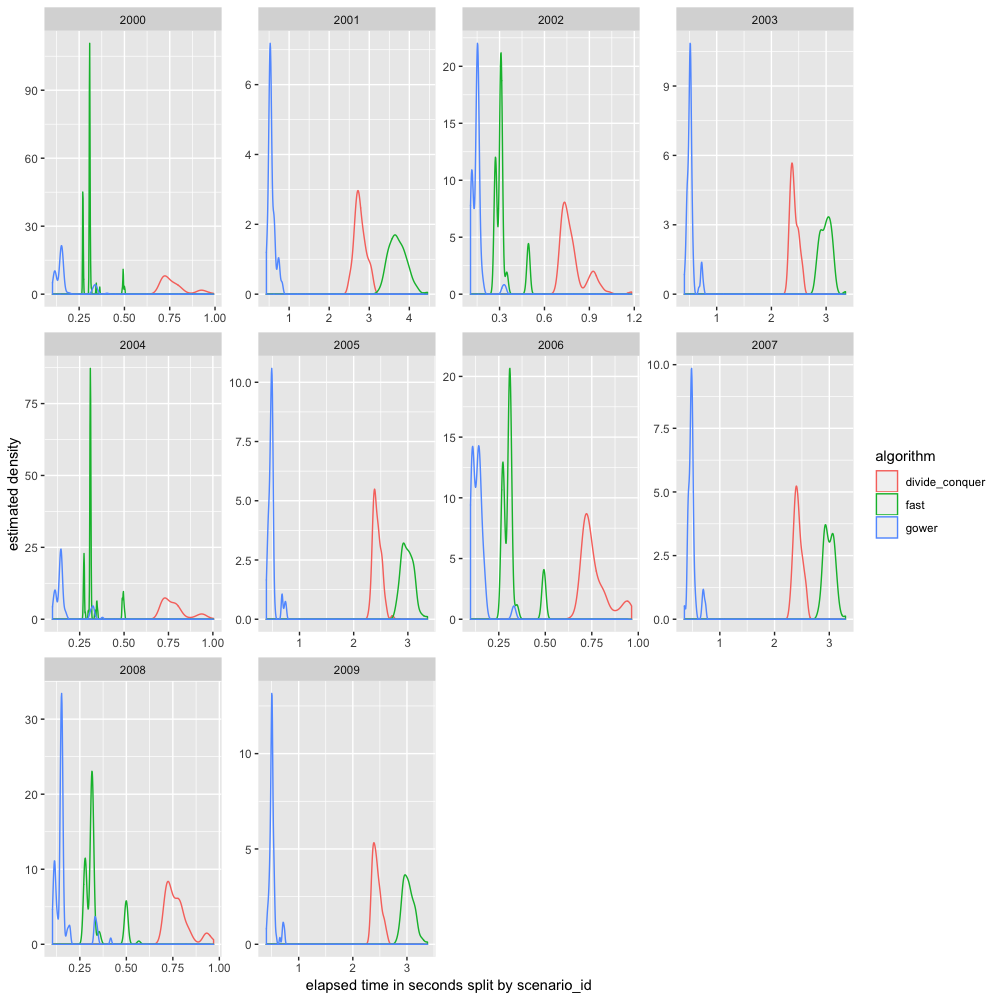
\includegraphics{./images/elapsed_time_3000.png}
    \caption{Elapsed time for each algorithm and each \textit{scenario\_id} of $n=3 \cdot 10^3$.}
    \label{elapsed_time_3000}
\end{figure}


\begin{figure}[!ht]
\centering
    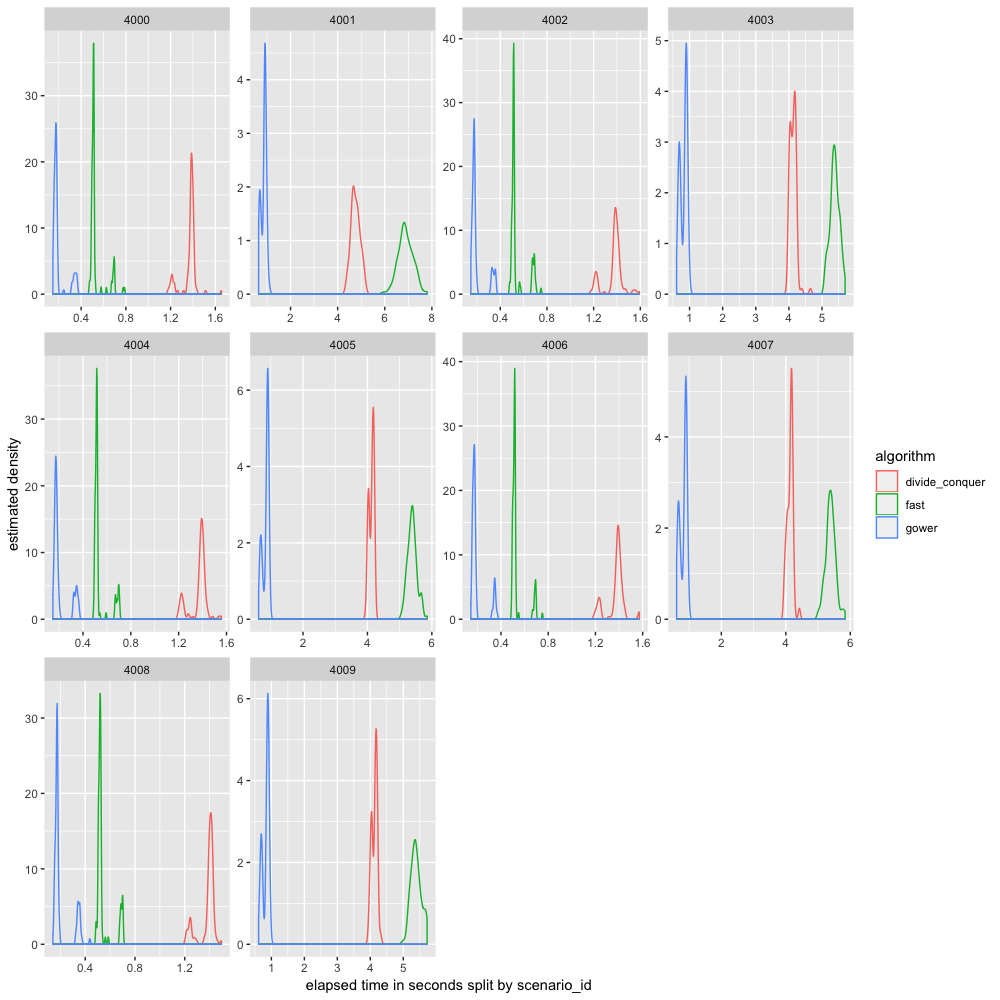
\includegraphics{./images/elapsed_time_5000.png}
    \caption{Elapsed time for each algorithm and each \textit{scenario\_id} of $n=5 \cdot 10^3$.}
    \label{elapsed_time_5000}
\end{figure}

\begin{figure}[!ht]
\centering
    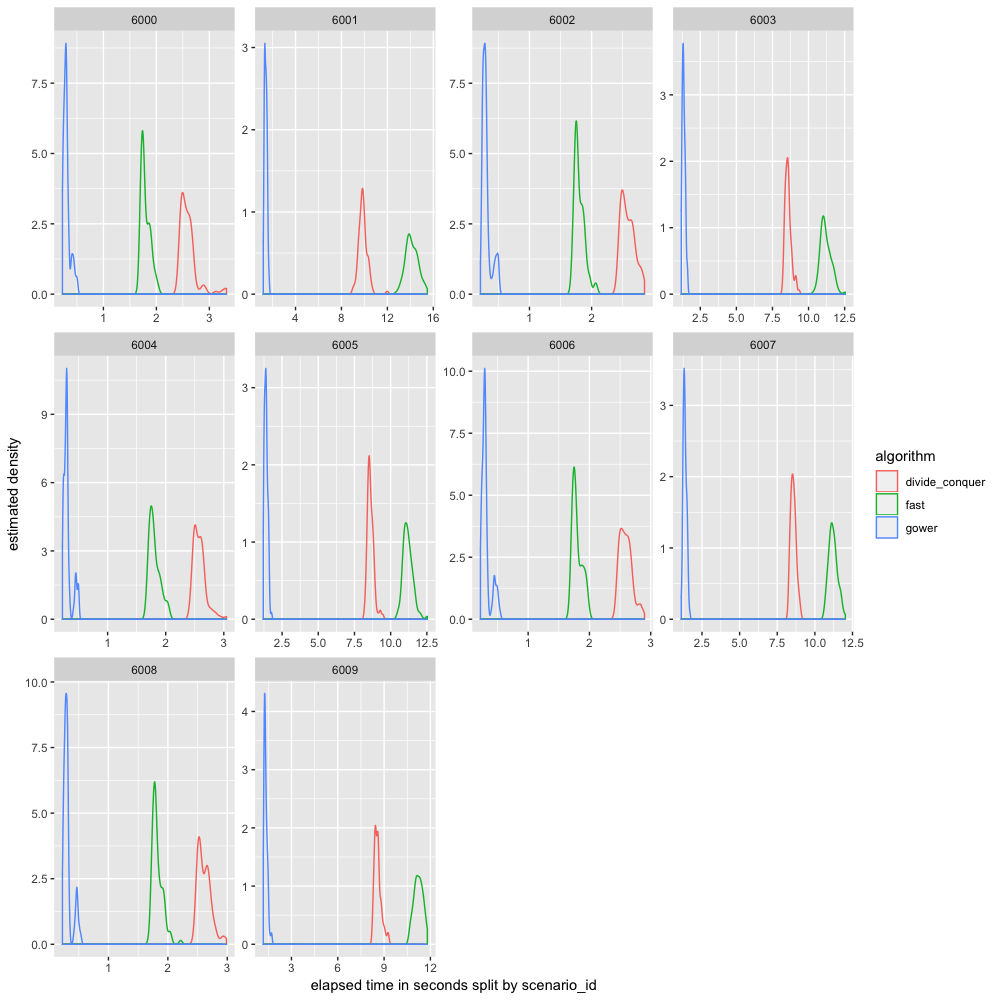
\includegraphics{./images/elapsed_time_10000.png}
    \caption{Elapsed time for each algorithm and each \textit{scenario\_id} of $n=10^4$.}
    \label{elapsed_time_10000}
\end{figure}

\begin{figure}[!ht]
\centering
    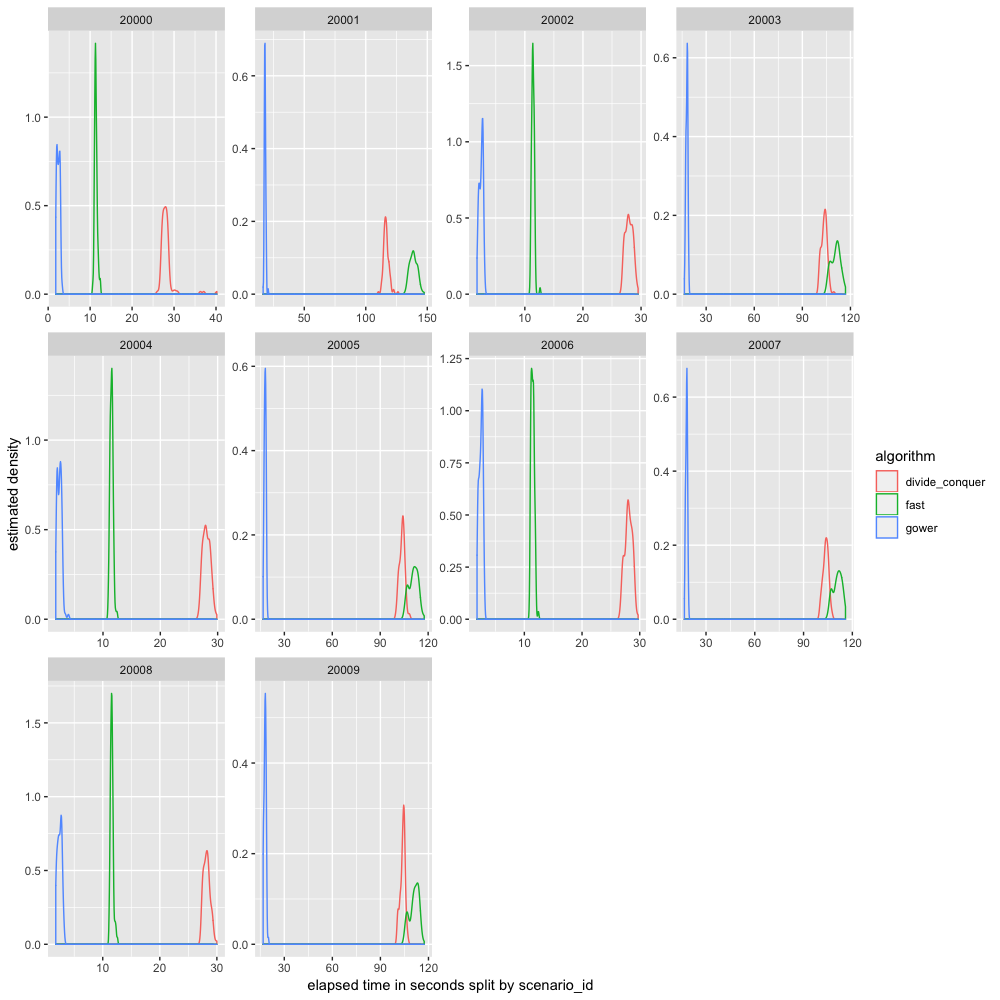
\includegraphics{./images/elapsed_time_100000.png}
    \caption{Elapsed time for each algorithm and each \textit{scenario\_id} of $n=10^5$.}
    \label{elapsed_time_100000}
\end{figure}

\begin{figure}[!ht]
\centering
    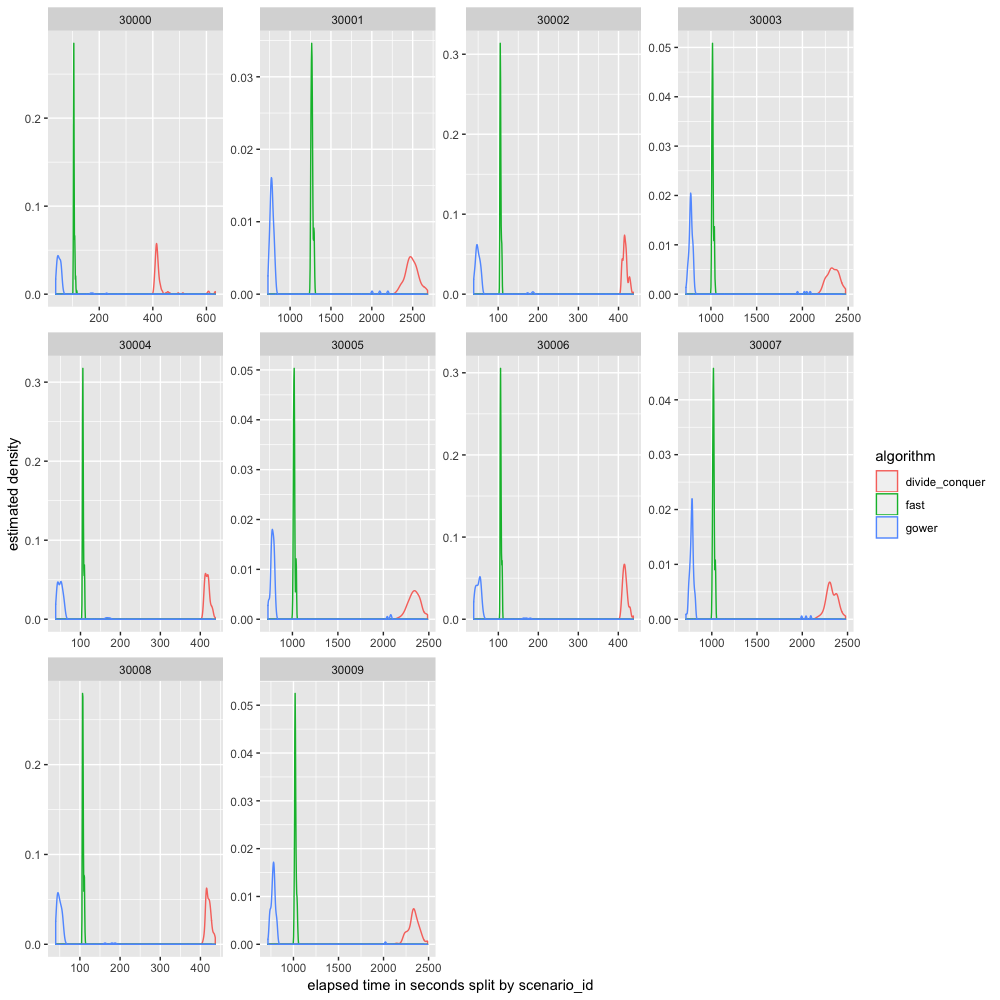
\includegraphics{./images/elapsed_time_1000000.png}
    \caption{Elapsed time for each algorithm and each \textit{scenario\_id} of $n=10^6$.}
    \label{elapsed_time_1000000}
\end{figure}

\FloatBarrier


\chapter{Code}
\label{chap:code}

\section{Divide and Conquer MDS}
\begin{lstlisting}
divide_conquer.mds <- function(
  x,
  l,
  s,
  metric
){
  
  # List positions
  ls_positions = list()
  list_eigenvalues = list()
  i_eigen = 1
  
  # Initial parameters
  p = ceiling(2*nrow(x)/l)
  groups = sample(x = p, size = nrow(x), replace = TRUE)
  groups = sort(groups)
  unique_group = unique(groups)
  total_groups = length(unique_group)
  
  for(k in 1:total_groups){
    # Getting the group that is being processed
    current_group = unique_group[k]
    x_positions_current_group = which(groups == current_group)
    ls_positions[[k]] = x_positions_current_group
    
    # Take the data in the following way:
    #   If it is the first iteration, take the data from first group
    #   else, take the data from k-1 and k groups
    if(k == 1){
      filter_rows_by_position = x_positions_current_group
      rows_processed = x_positions_current_group
    }else{
      
      rows_processed = c(
        rows_processed,
        x_positions_current_group
      )
      previous_group = unique_group[k-1]
      x_positions_previous_group =  which(groups == previous_group)
      
      # Rows to be filtered
      filter_rows_by_position = c(
        x_positions_previous_group,
        x_positions_current_group
      )
      
    }
    
    # Matrix to apply MDS
    submatrix_data = x[filter_rows_by_position, ]
    
    # Calculate distance
    distance_matrix = cluster::daisy(
      x = submatrix_data,
      metric = metric
    )
    
    # Applying MDS to the submatrix of data
    cmd_eig = stats::cmdscale(
      d = distance_matrix, 
      k = s,
      eig = TRUE
    )
    
    mds_iteration = cmd_eig$points
    if(p%%2 == 0){
      if(k%%2 == 0){
        list_eigenvalues[[i_eigen]] = cmd_eig$eig/nrow(submatrix_data)
        i_eigen = i_eigen + 1
      }
    }else{
      if(k %% 2 == 1){
        list_eigenvalues[[i_eigen]] = cmd_eig$eig/nrow(submatrix_data)
        i_eigen = i_eigen + 1
      }
    }

        row.names(mds_iteration) = row.names(submatrix_data)
    
    if(k == 1){
      # Define cum-MDS as MDS(1)
      cum_mds = mds_iteration
      
    }else{
      # Take the result of MDS(k-1) obtained with k-1 and k
      rn_prev = row.names(x)[x_positions_previous_group]  
      rn_cur = row.names(x)[x_positions_current_group] 
      pos_previous_group_current_mds = row.names(mds_iteration) %in% rn_prev 
      pos_current_group_current_mds = row.names(mds_iteration) %in% rn_cur
      mds_previous = mds_iteration[pos_previous_group_current_mds,]  
      mds_current = mds_iteration[pos_current_group_current_mds,]
      
      # From cum-MDS take the result of group k-1
      positions_cum_sum_previous = which(row.names(cum_mds) %in% rn_prev
      cum_mds_previous = cum_mds[positions_cum_sum_previous, ] 
      
      
      # Apply Procrustes transformation
      procrustes_result =  MCMCpack::procrustes(
        X = mds_previous, #The matrix to be transformed
        Xstar = cum_mds_previous, # target matrix
        translation = TRUE, 
        dilation = TRUE
      )
      
      rotation_matrix = procrustes_result$R
      dilation = procrustes_result$s
      translation = procrustes_result$tt
      ones_vector = rep(1, nrow(mds_current)) 
      translation_matrix = ones_vector %*% t(translation)
      
      # Transform the data for the k-th group  
      cum_mds_current = dilation * mds_current %*% rotation_matrix + 
        translation_matrix
      
      cum_mds = rbind(
        cum_mds,
        cum_mds_current
      )
      
    }
    
  }
  
  # Reordering
  reording_permutation = match(1:nrow(x), rows_processed)
  cum_mds = cum_mds[reording_permutation, ]
  
  
  return(
    list(
      points = cum_mds,
      eig = list_eigenvalues 
    )
  )
}
\end{lstlisting}


\section{Fast MDS}
\begin{lstlisting}
fast_mds <- function(
  x,
  l,
  s,
  k,
  metric
){
  
  # Initial parameters
  list_matrix = list()
  list_index = list()
  list_mds = list()
  list_mds_align = list()
  
  sub_sample_size = k * s
  n = nrow(x)
  
  # Division into p matrices
  # When doing the partitions it can happen that there are so many matrices
  # that s*k < nrow(x_i). In this case, we do a sampling again

  p = ceiling(l/sub_sample_size)
  observations_division = sample(x = p, size = nrow(x), replace = TRUE)
  observations_division = sort(observations_division)
  min_sample_size = min(table(observations_division))
  
  while( min_sample_size < sub_sample_size && p > 1){
    p = p - 1 
    observations_division = sample(x = p, size = nrow(x), replace = TRUE)
    observations_division = sort(observations_division)
    min_sample_size = min(table(observations_division))
  }
  
  
  
  # Partition into p submatrices
  for(i_group in 1:p){
    ind = which(observations_division == i_group)
    list_matrix[[i_group]] = x[ind, ]
  }
  
  able_to_do_mds = n/p <= l | p == 1
  
  
  # We can do MDS
  if(able_to_do_mds == TRUE){
    message(paste0("Non-recursive!!"))
    for (i_group in 1:p) {
      
      matrix_filter = list_matrix[[i_group]]
    
      # MDS for each submatrix
      distance_matrix = daisy(
        x = matrix_filter,
        metric = metric
      )
      
      list_mds[[i_group]] = stats::cmdscale(
        d = distance_matrix, 
        k = s
      )
      
      
      # Subsample
      sample_size = sub_sample_size
      if(sample_size > length( row.names(matrix_filter ) ) ){
        sample_size = length( row.names(matrix_filter ) )
      }
      
      
      list_index[[i_group]] = sample(
        x = row.names(matrix_filter), 
        size = sample_size, 
        replace = FALSE
      )
      
      
      # Building x_M_align
      ind_M = which(row.names(x) %in% list_index[[i_group]])
      if(i_group == 1){
        x_M_align = x[ind_M, ]
      }else{
        x_M_align = rbind(
          x_M_align,
          x[ind_M, ]
        )
      }
      
    }
    
    # M_align: MDS over x_M_align
    distance_matrix_M = distance_matrix = daisy(
      x = x_M_align,
      metric = metric
    )
    
    M_align = stats::cmdscale(
      d = distance_matrix_M, 
      k = s
    )
    
    # Global alignment
    for(i_group in 1:p){
      row_names = list_index[[i_group]]
      
      ind_M = which(row.names(M_align) %in% row_names)
      M_align_filter =  M_align[ind_M, ]
      
      di = list_mds[[i_group]]
      ind_mds = which(row.names( di ) %in% row_names)
      di_filter = di[ind_mds, ]
      
      # Alignment
      procrustes_result =  MCMCpack::procrustes(
        X = di_filter, #The matrix to be transformed
        Xstar = M_align_filter, # target matrix
        translation = TRUE, 
        dilation = TRUE
      )
      
      rotation_matrix = procrustes_result$R
      dilation = procrustes_result$s
      translation = procrustes_result$tt
      ones_vector = rep(1, nrow(di)) 
      translation_matrix = ones_vector %*% t(translation)
      
      
      tranformation_di = dilation * di %*% rotation_matrix + translation_matrix
      
      
      # Append
      if(i_group == 1){
        Z = tranformation_di
      } else{
        Z = rbind(
          Z,
          tranformation_di
        )
        
      }
    }
    
    row.names(Z) = row.names(x)
    
  }else{
    message("Recursive!!!")
    list_zi <- list()
    list_index <- list()
    
    for(i_group in 1:p){
      # Apply the algorithm
      list_zi[[i_group]] = fast_mds(
        x = list_matrix[[i_group]],
        n = nrow(list_matrix[[i_group]]),
        l = l,
        s = s,
        k = k,
        metric = metric 
      )
      
      #Take a subsample
      list_index[[i_group]] = sample(
        x = row.names( list_zi[[i_group]] ), 
        size = k * s, 
        replace = FALSE
      )
      
      ind = which( row.names( list_zi[[i_group]] ) %in% list_index[[i_group]])
      submatrix = list_matrix[[i_group]][ind, ] 
    
      
      if(i_group == 1){
        x_M_align = submatrix 
      } else{
        x_M_align = rbind(
          x_M_align,
          submatrix
        )
      }
    }
    
    message(paste0("        At the end x_M_align has ", nrow(x_M_align), " rows"))
    
   
    distance_matrix_M  = daisy(
      x = x_M_align,
      metric = metric
    )
    
    M_align = stats::cmdscale(
      d = distance_matrix_M, 
      k = s
    )
    
    
    # Global alignment
    for(i_group in 1:p){
      row_names = list_index[[i_group]]
      
      ind_M = which(row.names(x_M_align) %in% row_names)
      M_align_filter =  M_align[ind_M, ]
      
      di = list_zi[[i_group]]
      ind_mds = which(row.names( di ) %in% row_names)
      di_filter = di[ind_mds, ]
      
      # Alignment
      procrustes_result =  MCMCpack::procrustes(
        X = di_filter, #The matrix to be transformed
        Xstar = M_align_filter, # target matrix
        translation = TRUE, 
        dilation = TRUE
      )
      
      rotation_matrix = procrustes_result$R
      dilation = procrustes_result$s
      translation = procrustes_result$tt
      ones_vector = rep(1, nrow(di)) 
      translation_matrix = ones_vector %*% t(translation)
      
      
      tranformation_di = dilation * di %*% rotation_matrix + translation_matrix
      
      
      # Append
      if(i_group == 1){
        Z = tranformation_di
      } else{
        Z = rbind(
          Z,
          tranformation_di
        )
        
      }
    }
    
    row.names(Z) = row.names(x)
      
  }
  
  return(
    list(
      Z = Z,
      eigenvalues = NA
    )
  )
}
\end{lstlisting}


\section{MDS based on Gower interpolation}
\begin{lstlisting}
gower.interpolation.mds <- function(
  x,
  l,
  s
){
  
  nrow_x = nrow(x)
  p = ceiling(nrow_x/l)
  if(p<1) p = 1
  
  if( p>1 ){
    # Do MDS with the first group and then use the Gower interpolation formula
    sample_distribution = sample(x = p, size = nrow_x, replace = TRUE)
    sample_distribution = sort(sample_distribution)
    
    # Get the first group 
    ind_1 = which(sample_distribution == 1)
    n_1 = length(ind_1)
    
    # Do MDS with the first group
    submatrix_data = x[ind_1, ]
    
    distance_matrix = cluster::daisy(
      x = submatrix_data,
      metric = "euclidean"
    )
    
    distance_matrix = as.matrix(distance_matrix)
    
    # MDS for the first group
    cmd_eig = stats::cmdscale(
      d = distance_matrix, 
      k = s,
      eig = TRUE
    )
    
    M = cmd_eig$points
    eigen = cmd_eig$eig/nrow(M)
    cum_mds = M
    
    # Calculations needed to do Gower interpolation
    delta_matrix = distance_matrix^2 
    In = diag(n_1)
    ones_vector = rep(1, n_1)
    J = In - 1/n_1*ones_vector %*% t(ones_vector)
    G = -1/2 * J %*% delta_matrix %*% t(J) 
    g_vector = diag(G)
    # S = cov(M)
    S = 1/(nrow(M)-1)*t(M) %*% M
    S_inv = solve(S)
    
    # For the rest of the groups, do the interpolation
    for(i_group in 2:p){
      # Filtering the data
      ind_i_group = which(sample_distribution == i_group)
      submatrix_data = x[ind_i_group, ]
      
      
      # A matrix
      distance_matrix_filter = pdist::pdist(
        X = submatrix_data,
        Y = x[ind_1, ]
      )
      
      distance_matrix_filter = as.matrix(distance_matrix_filter)
      A = distance_matrix_filter^2
      ones_vector = rep(1, length(ind_i_group))
      MDS_i_group = 1/(2*n_1)*(ones_vector %*%t(g_vector) - A) %*% M %*% S_inv
      cum_mds = rbind(
        cum_mds,
        MDS_i_group
      )
    }
  }else{
    # It is possible to run MDS directly
    distance_matrix = cluster::daisy(
      x = x,
      metric = "euclidean"
    )
    
    distance_matrix = as.matrix(distance_matrix)
    
    # MDS for the first groups
    cmd_eig = stats::cmdscale(
      d = distance_matrix, 
      k = s,
      eig = TRUE
    )
    
    cum_mds = cmd_eig$points
    eigen = cmd_eig$eig/nrow_x
  }
  
  return(
    list(
      points = cum_mds,
      eig = eigen
    )
  )
}

\end{lstlisting}
\end{document}
